\documentclass[aspectratio=43]{beamer}
\usepackage[spanish]{babel}
\setbeamertemplate{caption}[numbered]
\usepackage{siunitx}
\sisetup{detect-all}
\usepackage{capt-of}
\usepackage{subcaption}   % para subfiguras modernas
% (opcional) tamaño de letras en captions
\captionsetup{font=footnotesize}


\input{chapters/preamble}
\title{Redes de Bravais} %->->->->-> Check hyperref title <-<-<-<-<-
\subtitle{Red ortorrómbica centrada en las bases}
\input{colores}
\author[Julio Alfredo Ballinas]{Julio Alfredo Ballinas García}
\institute[FCFM]{
    Estado sólido%
    \\%
    Dra. Ana Lilia Gonzalez Ronquillo%
} %You can change the Institution if you are from somewhere else
\date{25 de agosto, 2025}
%\logo{
\includegraphics[width= 0.2\textwidth]{images/a-logo.png}}

\begin{document}
   
    \frame{\titlepage}
    
    \begin{frame}{Índice}
        \tableofcontents
    \end{frame}
    
 \section{Diamante}
    
    \frame{\sectionpage}
    
    \begin{frame}{Estructura del diamante}
  \begin{itemize}
 Según Kittel el diamante es una forma cristalina del carnono, la cual se forma debido al proceso de 
  \end{itemize}
\end{frame}

\begin{frame}{August Bravais}
 \begin{figure}
    \centering
    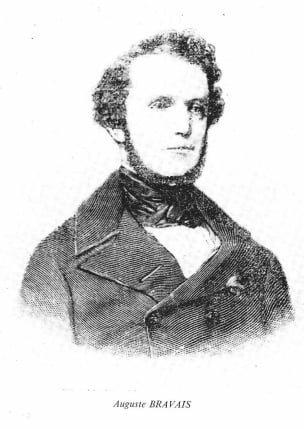
\includegraphics[width=0.3\linewidth]{images/august_bravais}
    \caption{August Bravais (1811–1863), pionero en la clasificación de las redes cristalinas.}
 \end{figure}
\end{frame}
  
\begin{frame}{Red cristalina}
  \begin{columns}
    \column{0.55\textwidth}
      \begin{itemize}
        \item Los átomos en un cristal no se disponen de forma aleatoria. 
        \item Siguen un \textbf{orden periódico} en el espacio. 
        \item Esta periodicidad es la que da lugar a las 
              \textbf{propiedades físicas} características de los sólidos cristalinos.
      \end{itemize}

    \column{0.45\textwidth}
      \centering
      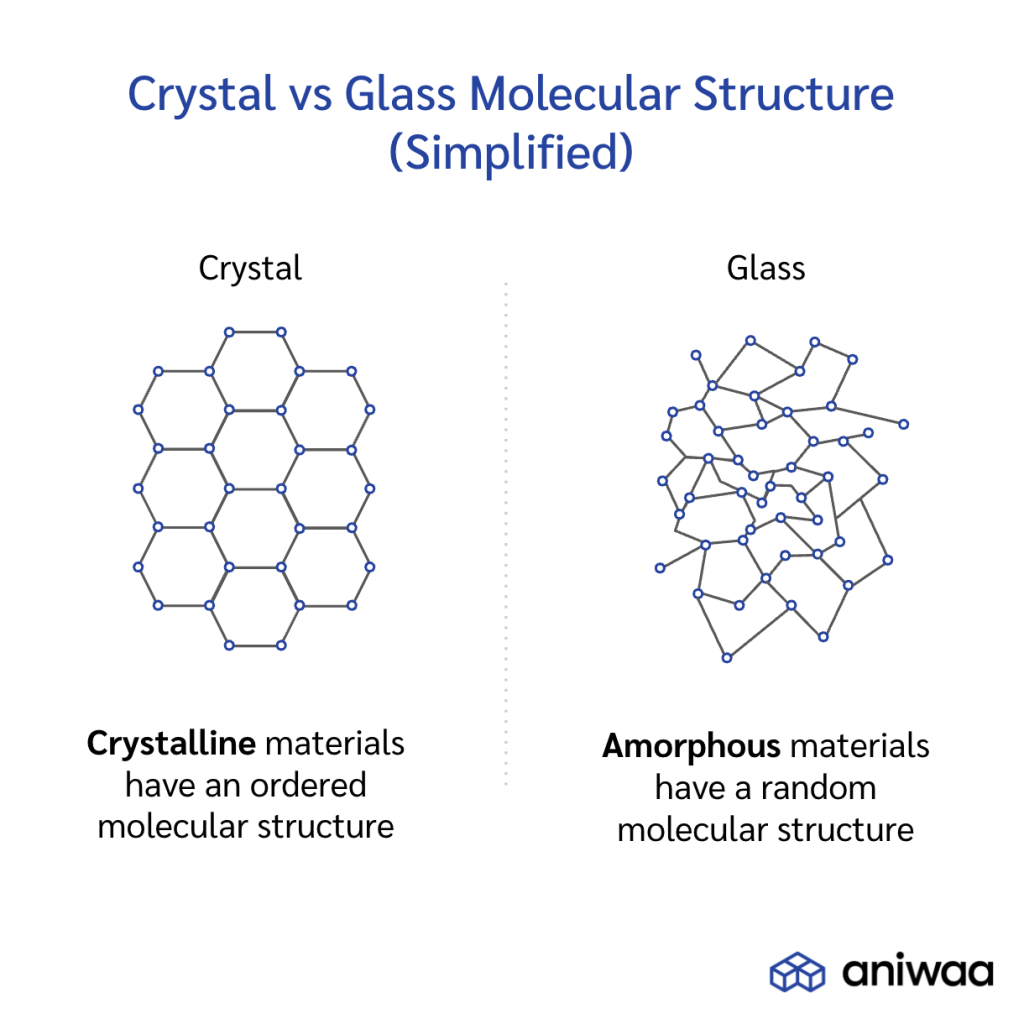
\includegraphics[width=\linewidth]{images/amorfoyno.png} % pon tu imagen aquí
      \captionof{figure}{Comparación entre sólido amorfo (izq.) y cristalino (der.).}
  \end{columns}
\end{frame}

\begin{frame}{Ejemplos de sólidos cristalinos (más comunes)}
  \begin{itemize}
    \item \textbf{Cloruro de sodio (NaCl)} — cristal iónico, red cúbica centrada en las caras.
    \item \textbf{Cuarzo (SiO$_2$)} — estructura trigonal/hexagonal, muy abundante en la corteza terrestre.
    \item \textbf{Grafito (C)} — aunque es otra forma del carbono, tiene estructura hexagonal en láminas.
    \item \textbf{Hielo (H$_2$O)} — en su forma cristalina hexagonal (hielo Ih).
      \item Materiales cuya regularidad superficial es reflejo de su simetría interna.
  \end{itemize}
\end{frame}

\begin{frame}{Ejemplos comunes de sólidos cristalinos}
  \begin{figure}
    \centering
    % Primera fila
    \begin{subfigure}{0.45\linewidth}
      \centering
      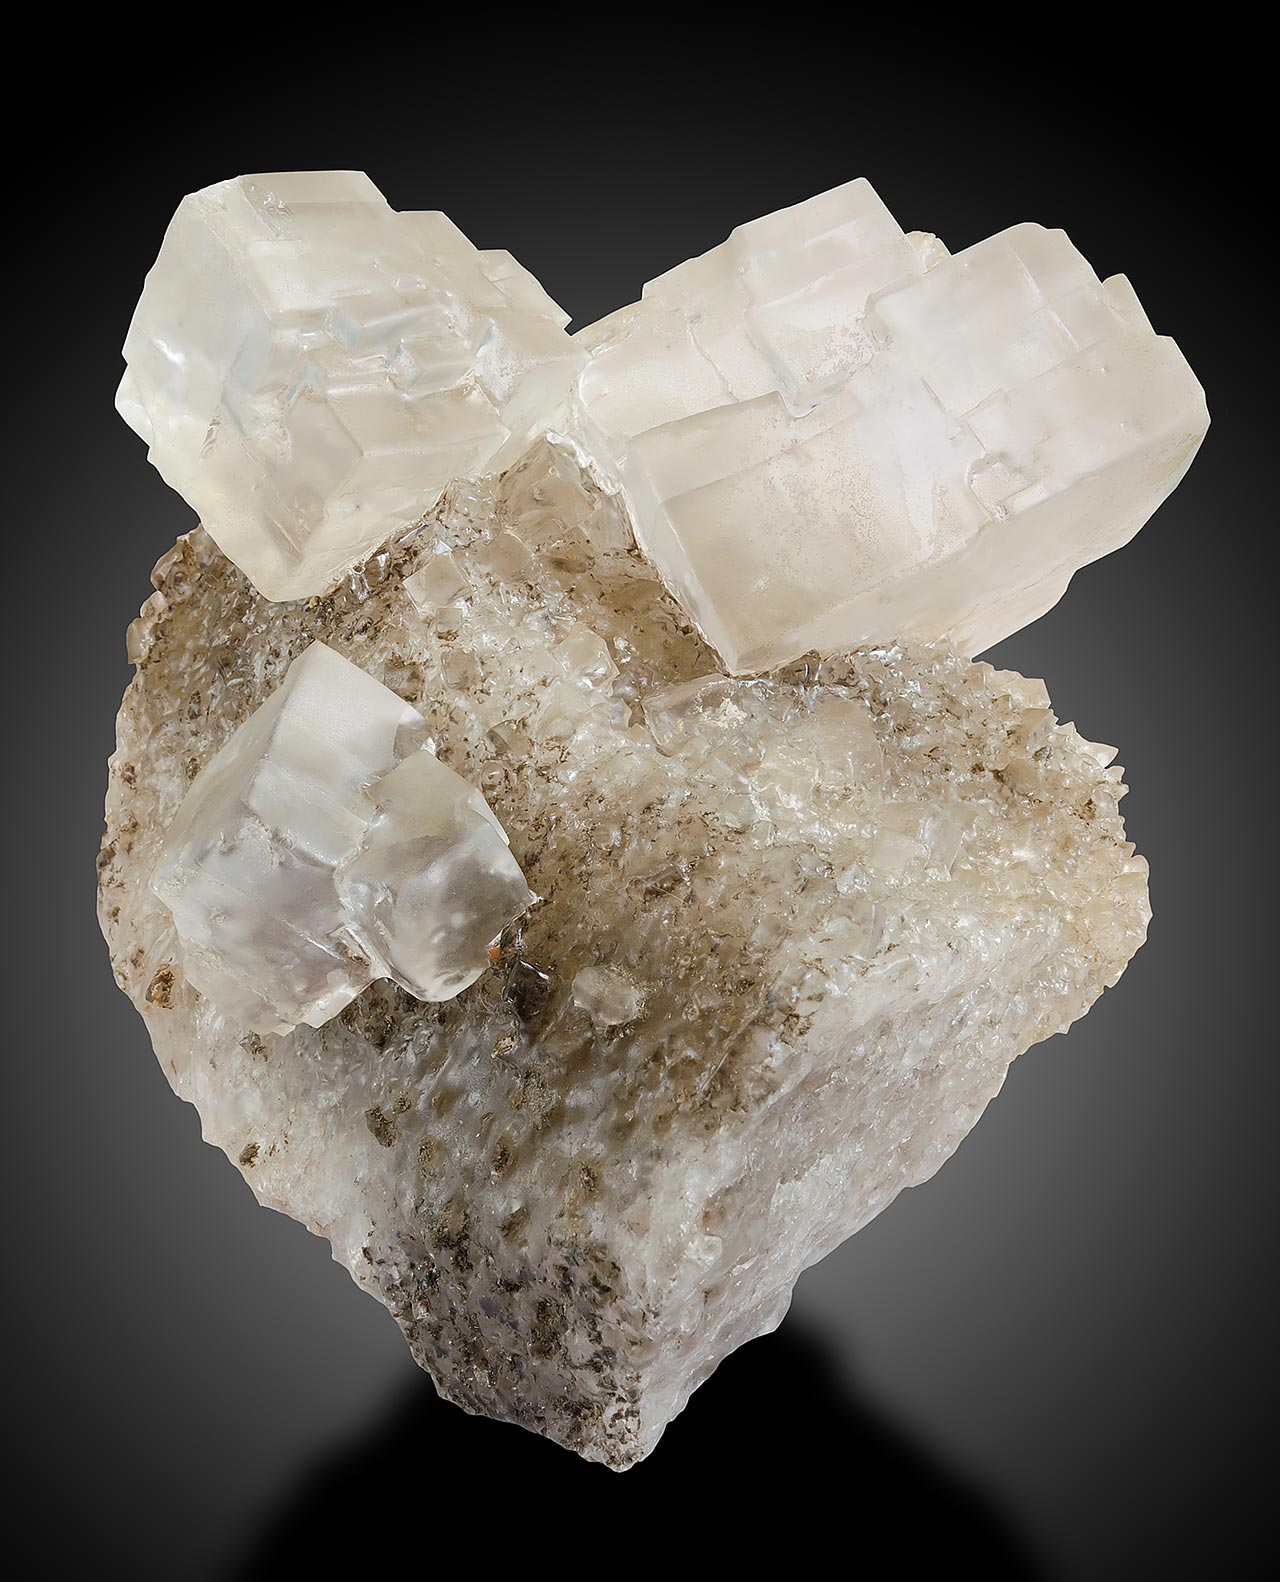
\includegraphics[width=\linewidth,height=2.5cm,keepaspectratio]{images/halita_natural.jpg}
      \caption{Halita (NaCl)}
    \end{subfigure}\hfill
    \begin{subfigure}{0.45\linewidth}
      \centering
      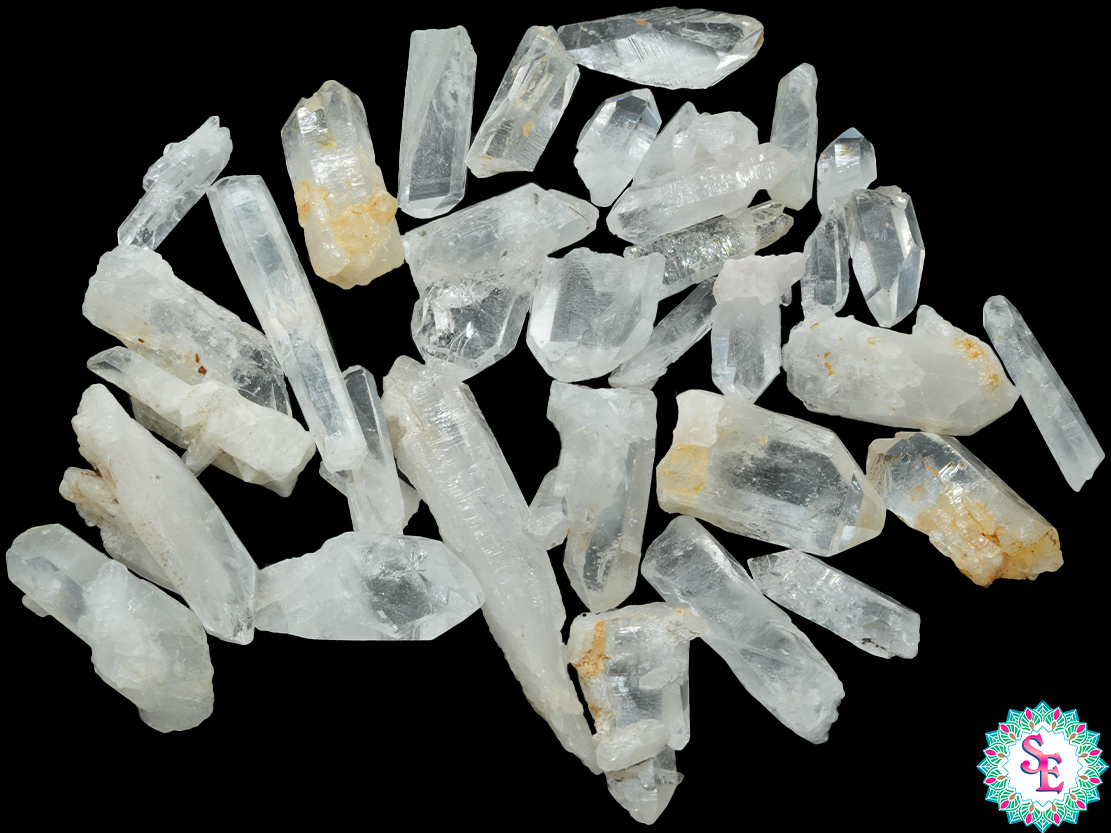
\includegraphics[width=\linewidth,height=2.5cm,keepaspectratio]{images/cuarzo_natural.jpg}
      \caption{Cuarzo (SiO$_2$)}
    \end{subfigure}

    \vspace{0.2cm}

    % Segunda fila
    \begin{subfigure}{0.45\linewidth}
      \centering
      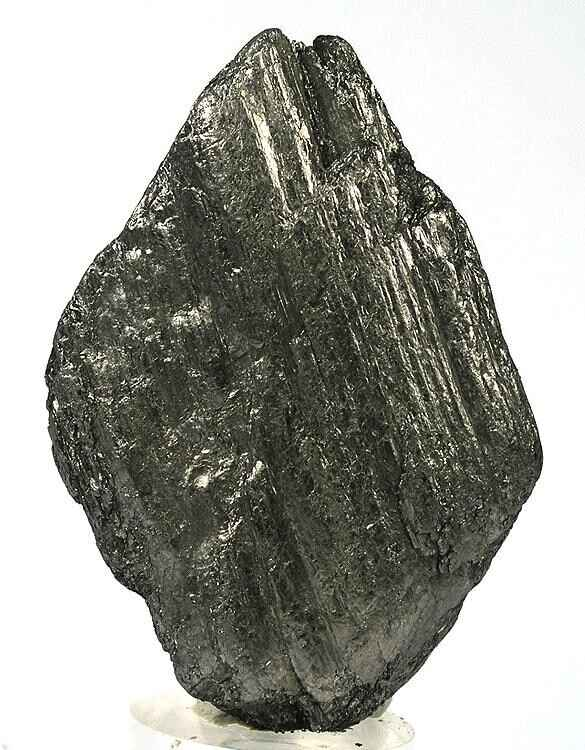
\includegraphics[width=\linewidth,height=2.5cm,keepaspectratio]{images/grafito.jpg}
      \caption{Grafito (C)}
    \end{subfigure}\hfill
    \begin{subfigure}{0.45\linewidth}
      \centering
      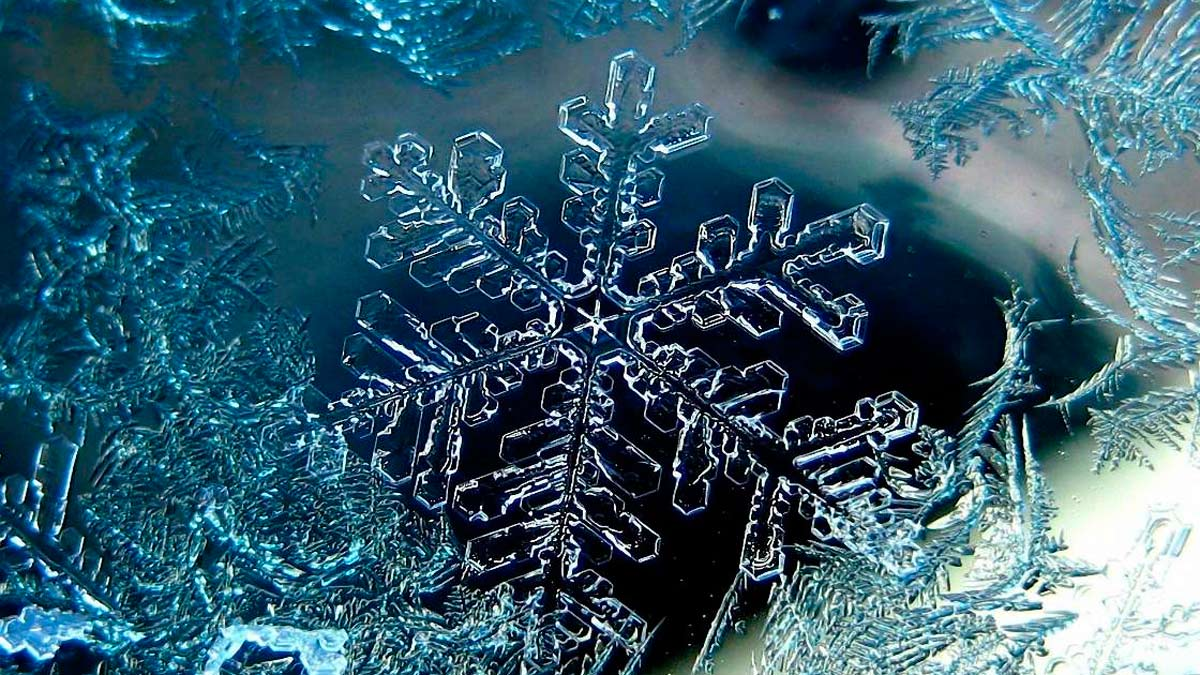
\includegraphics[width=\linewidth,height=2.5cm,keepaspectratio]{images/hielo_hexagonal.jpg}
      \caption{Hielo Ih (H$_2$O)}
    \end{subfigure}
  \end{figure}
\end{frame}


\begin{frame}{Ejemplos de sólidos cristalinos (gemas)}
  \begin{itemize}
   \item \textbf{Diamante (C)} — red covalente cúbica tipo diamante, dureza máxima (10 Mohs).
    \item \textbf{Zafiro (Al$_2$O$_3$)} — variedad azul del corindón, sistema trigonal.
    \item \textbf{Rubí (Al$_2$O$_3$)} — corindón rojo, por impurezas de cromo.
    \item \textbf{Esmeralda (Be$_3$Al$_2$(SiO$_3$)$_6$)} — variedad verde del berilo, sistema hexagonal.
    \item \textbf{Topacio (Al$_2$SiO$_4$(F,OH)$_2$)} — ortorrómbico, gemas amarillas y azules.
    \item \textbf{Amatista (SiO$_2$)} — variedad violeta del cuarzo.
  \end{itemize}
\end{frame}

\begin{frame}{Ejemplos de sólidos cristalinos (gemas)}
  \begin{figure}
    \centering
    % Primera fila
    \begin{subfigure}{0.30\linewidth}
      \centering
      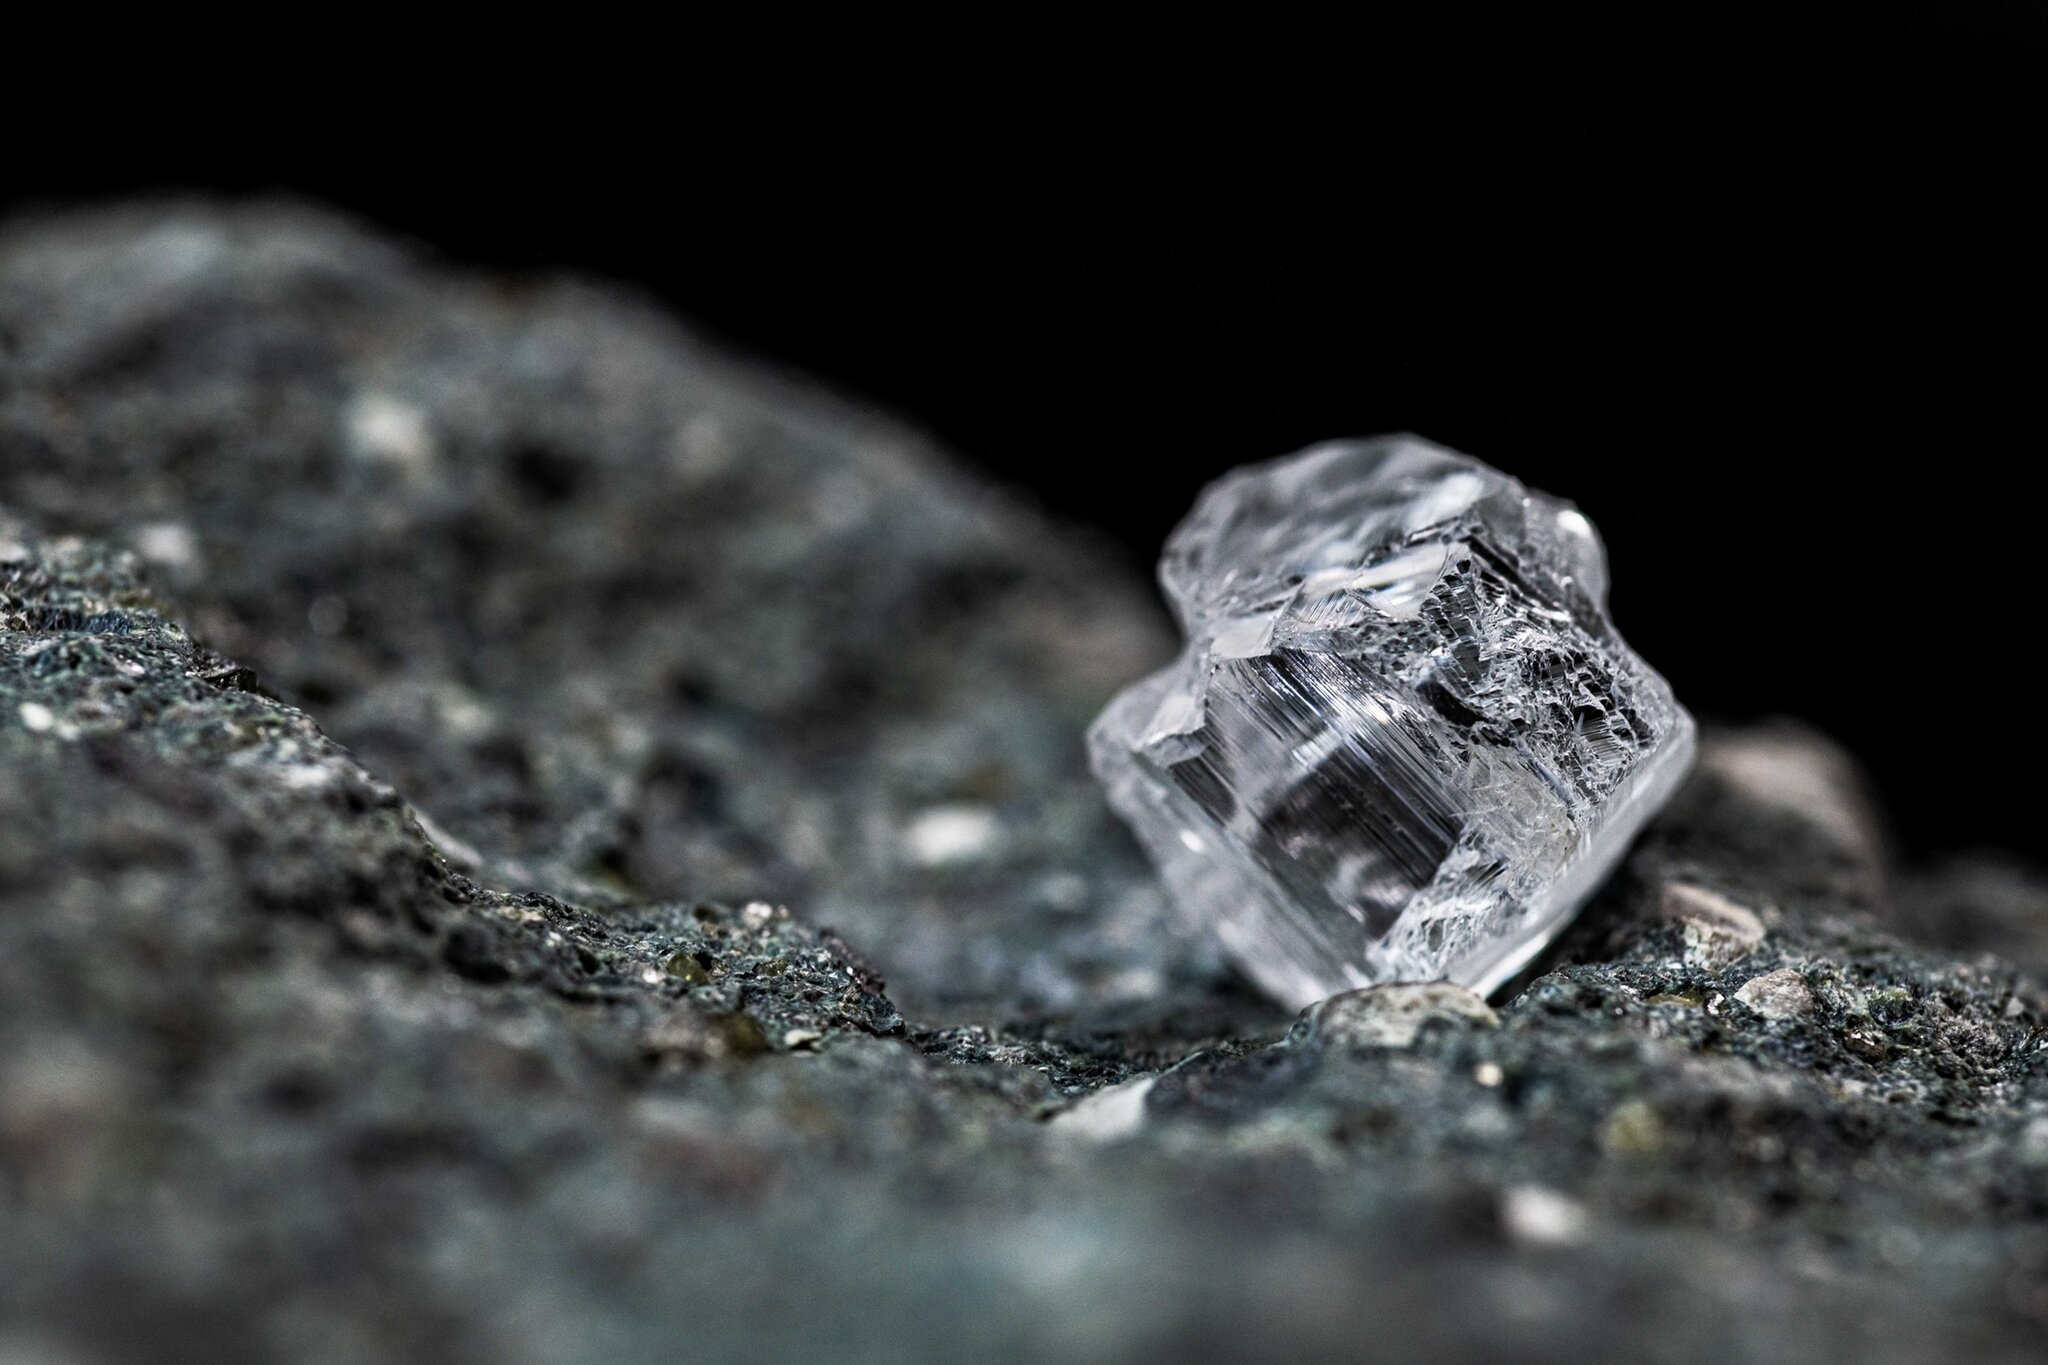
\includegraphics[width=\linewidth,height=2.5cm,keepaspectratio]{images/diamante.jpg}
      \caption{Diamante (C)}
    \end{subfigure}\hfill
    \begin{subfigure}{0.30\linewidth}
      \centering
      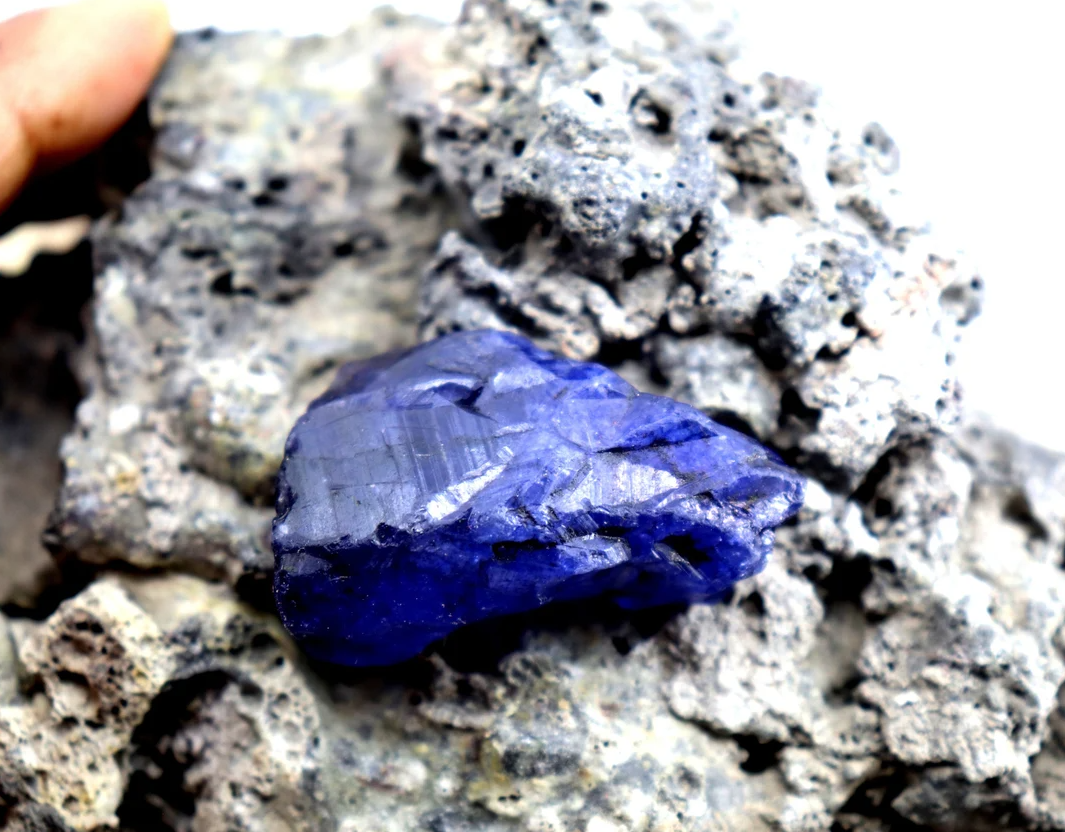
\includegraphics[width=\linewidth,height=2.5cm,keepaspectratio]{images/zafiro.png}
      \caption{Zafiro (Al$_2$O$_3$)}
    \end{subfigure}\hfill
    \begin{subfigure}{0.30\linewidth}
      \centering
      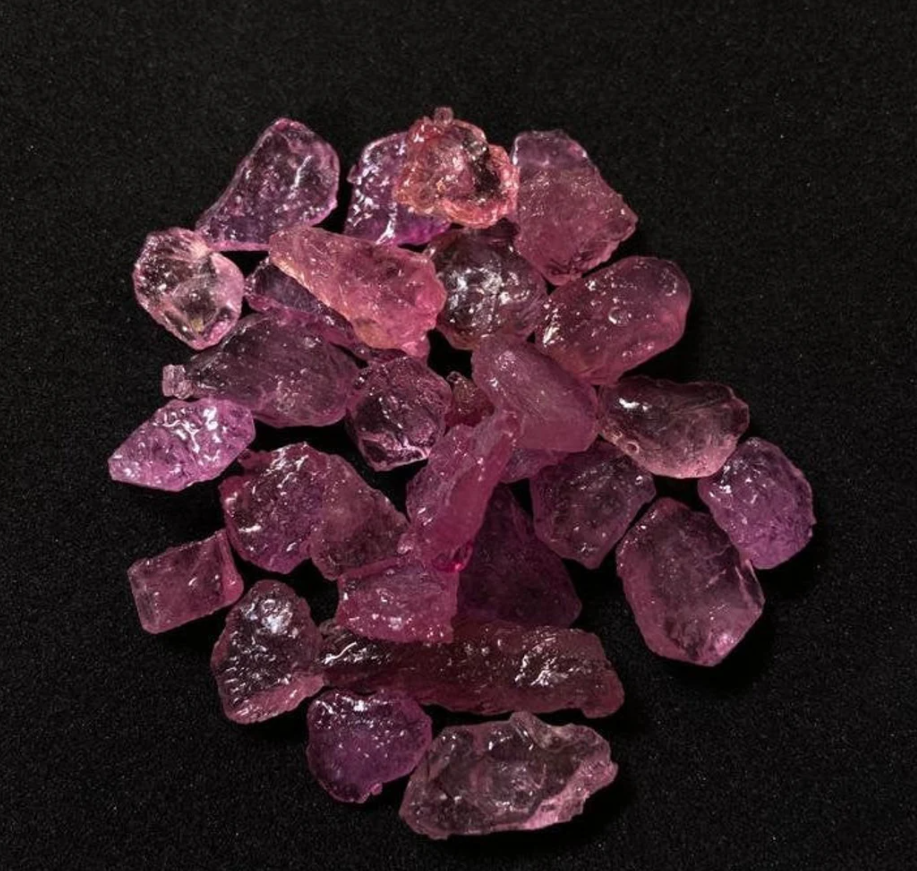
\includegraphics[width=\linewidth,height=2.5cm,keepaspectratio]{images/rubi.png}
      \caption{Rubí (Al$_2$O$_3$)}
    \end{subfigure}

    \vspace{0.3cm}

    % Segunda fila
    \begin{subfigure}{0.30\linewidth}
      \centering
      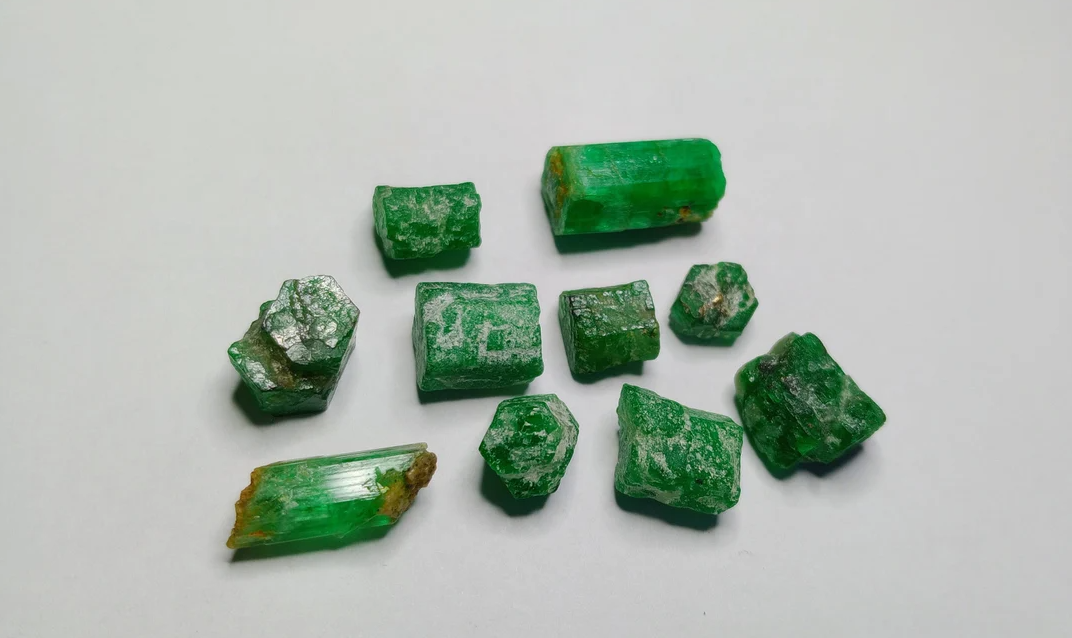
\includegraphics[width=\linewidth,height=2.5cm,keepaspectratio]{images/esmeralda.png}
      \caption{Esmeralda (Be$_3$Al$_2$(SiO$_3$)$_6$)}
    \end{subfigure}\hfill
    \begin{subfigure}{0.30\linewidth}
      \centering
      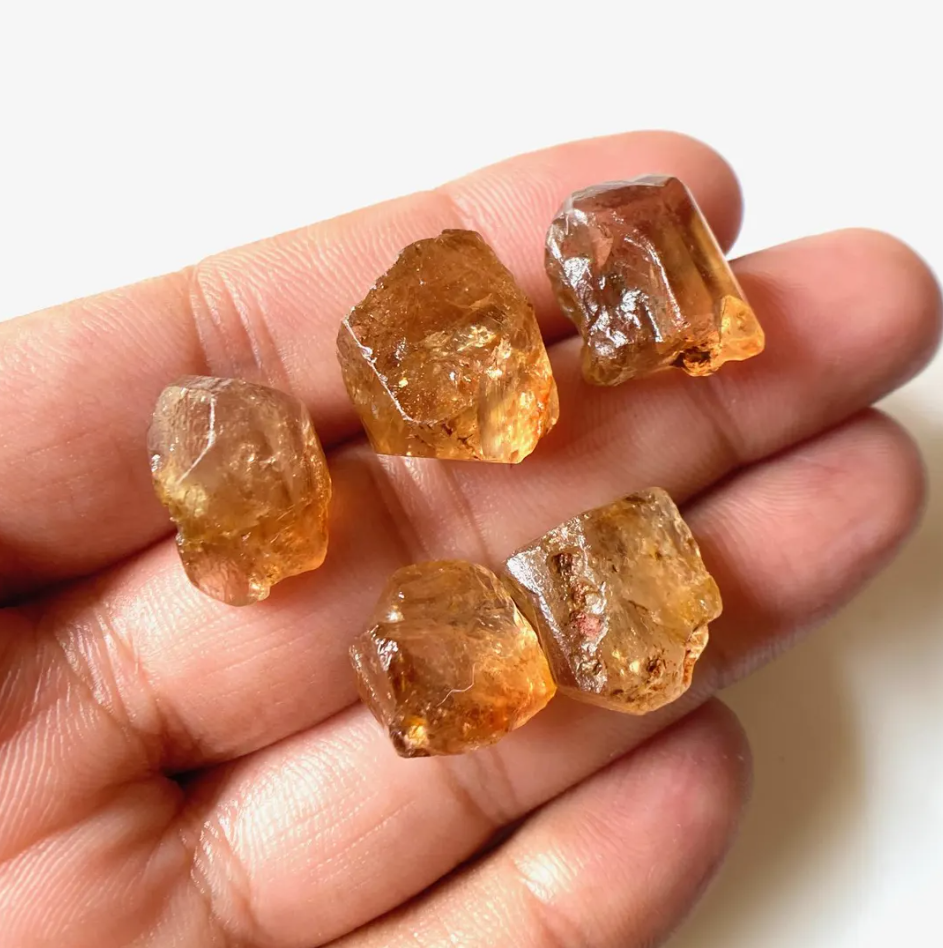
\includegraphics[width=\linewidth,height=2.5cm,keepaspectratio]{images/topacio.png}
      \caption{Topacio (Al$_2$SiO$_4$(F,OH)$_2$)}
    \end{subfigure}\hfill
    \begin{subfigure}{0.30\linewidth}
      \centering
      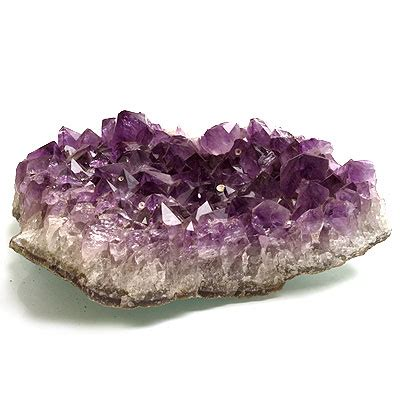
\includegraphics[width=\linewidth,height=2.5cm,keepaspectratio]{images/amatista.jpeg}
      \caption{Amatista (SiO$_2$)}
    \end{subfigure}
  \end{figure}
\end{frame}


\begin{frame}{Ejemplos de sólidos cristalinos (metálicos)}
  \begin{itemize}
    \item \textbf{Pirita (FeS$_2$)} — “oro de los tontos”, sistema cúbico.
    \item \textbf{Magnetita (Fe$_3$O$_4$)} — magnética, sistema isométrico.
    \item \textbf{Galena (PbS)} — mena principal del plomo, estructura cúbica.
    \item \textbf{Hematita (Fe$_2$O$_3$)} — óxido de hierro, sistema trigonal.
    \item \textbf{Cobre (Cu)} — red metálica cúbica centrada en las caras.
    \item \textbf{Hierro (Fe)} — red metálica cúbica centrada en el cuerpo (a altas T cambia).
  \end{itemize}
\end{frame}

\begin{frame}{Ejemplos de sólidos cristalinos (metálicos)}
  \begin{figure}
    \centering
    % Primera fila
    \begin{subfigure}{0.30\linewidth}
      \centering
      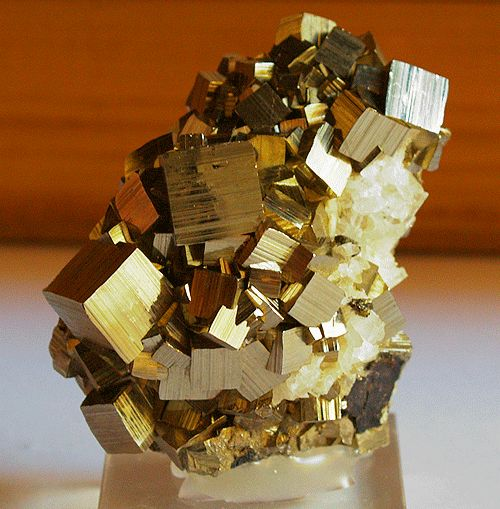
\includegraphics[width=\linewidth,height=3cm,keepaspectratio]{images/pirita.jpg}
      \caption{Pirita (FeS$_2$)}
    \end{subfigure}\hfill
    \begin{subfigure}{0.30\linewidth}
      \centering
      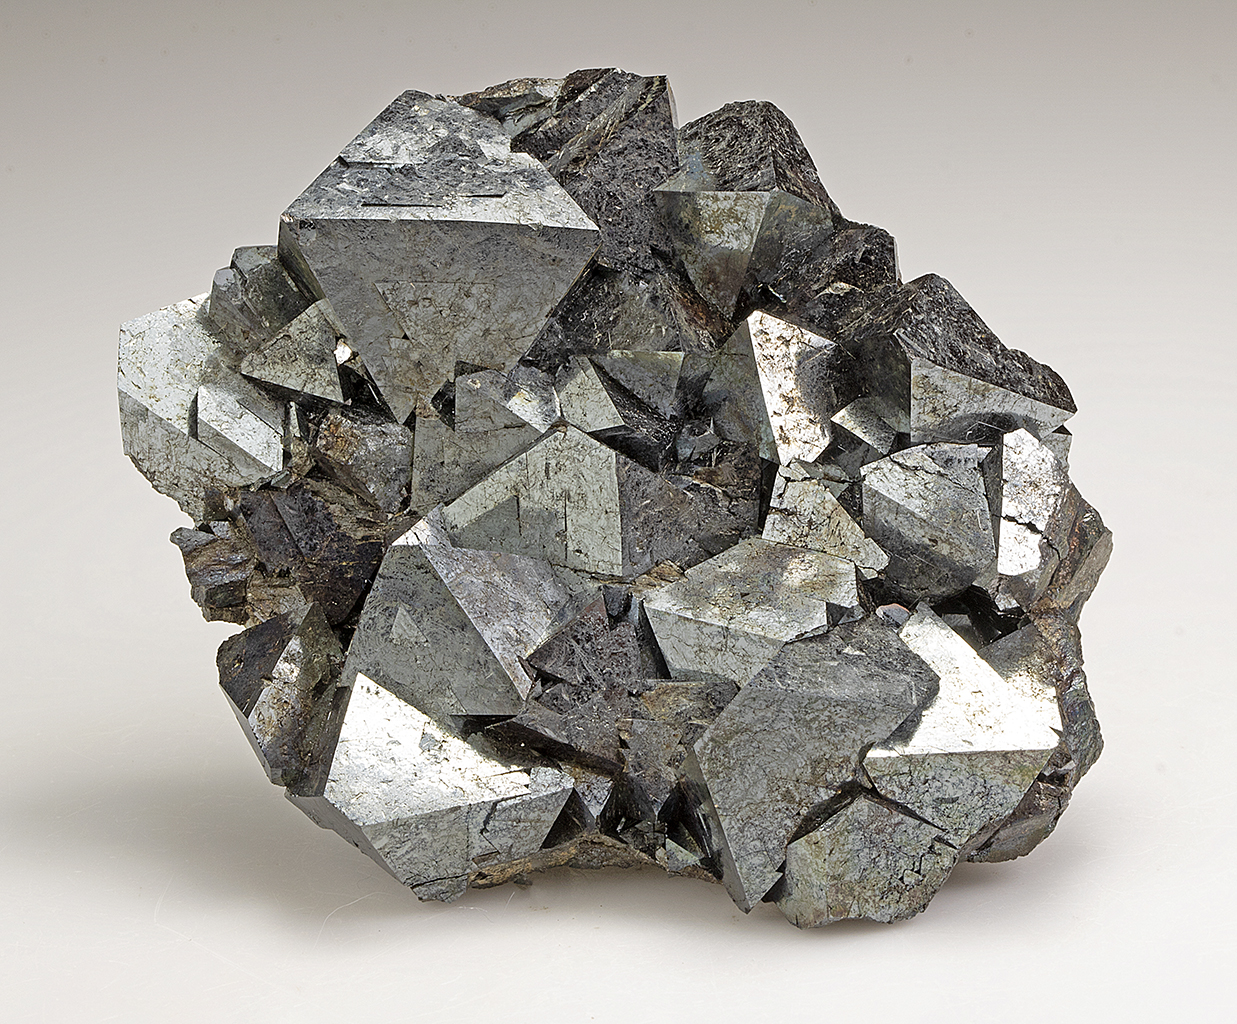
\includegraphics[width=\linewidth,height=3cm,keepaspectratio]{images/magnetita.jpg}
      \caption{Magnetita (Fe$_3$O$_4$)}
    \end{subfigure}\hfill
    \begin{subfigure}{0.30\linewidth}
      \centering
      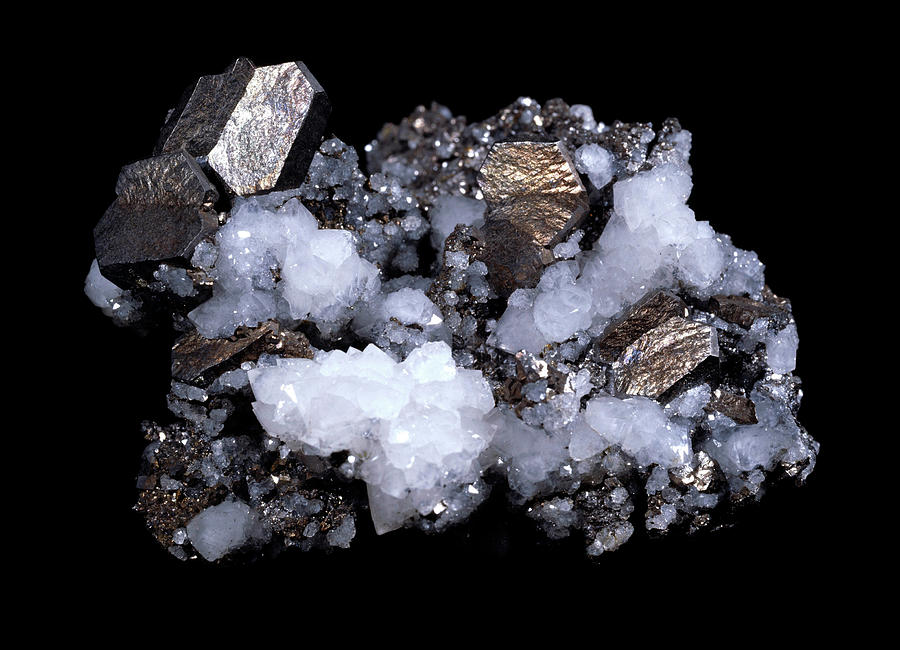
\includegraphics[width=\linewidth,height=3cm,keepaspectratio]{images/galena.jpg}
      \caption{Galena (PbS)}
    \end{subfigure}

    \vspace{0.3cm}

    % Segunda fila
    \begin{subfigure}{0.30\linewidth}
      \centering
      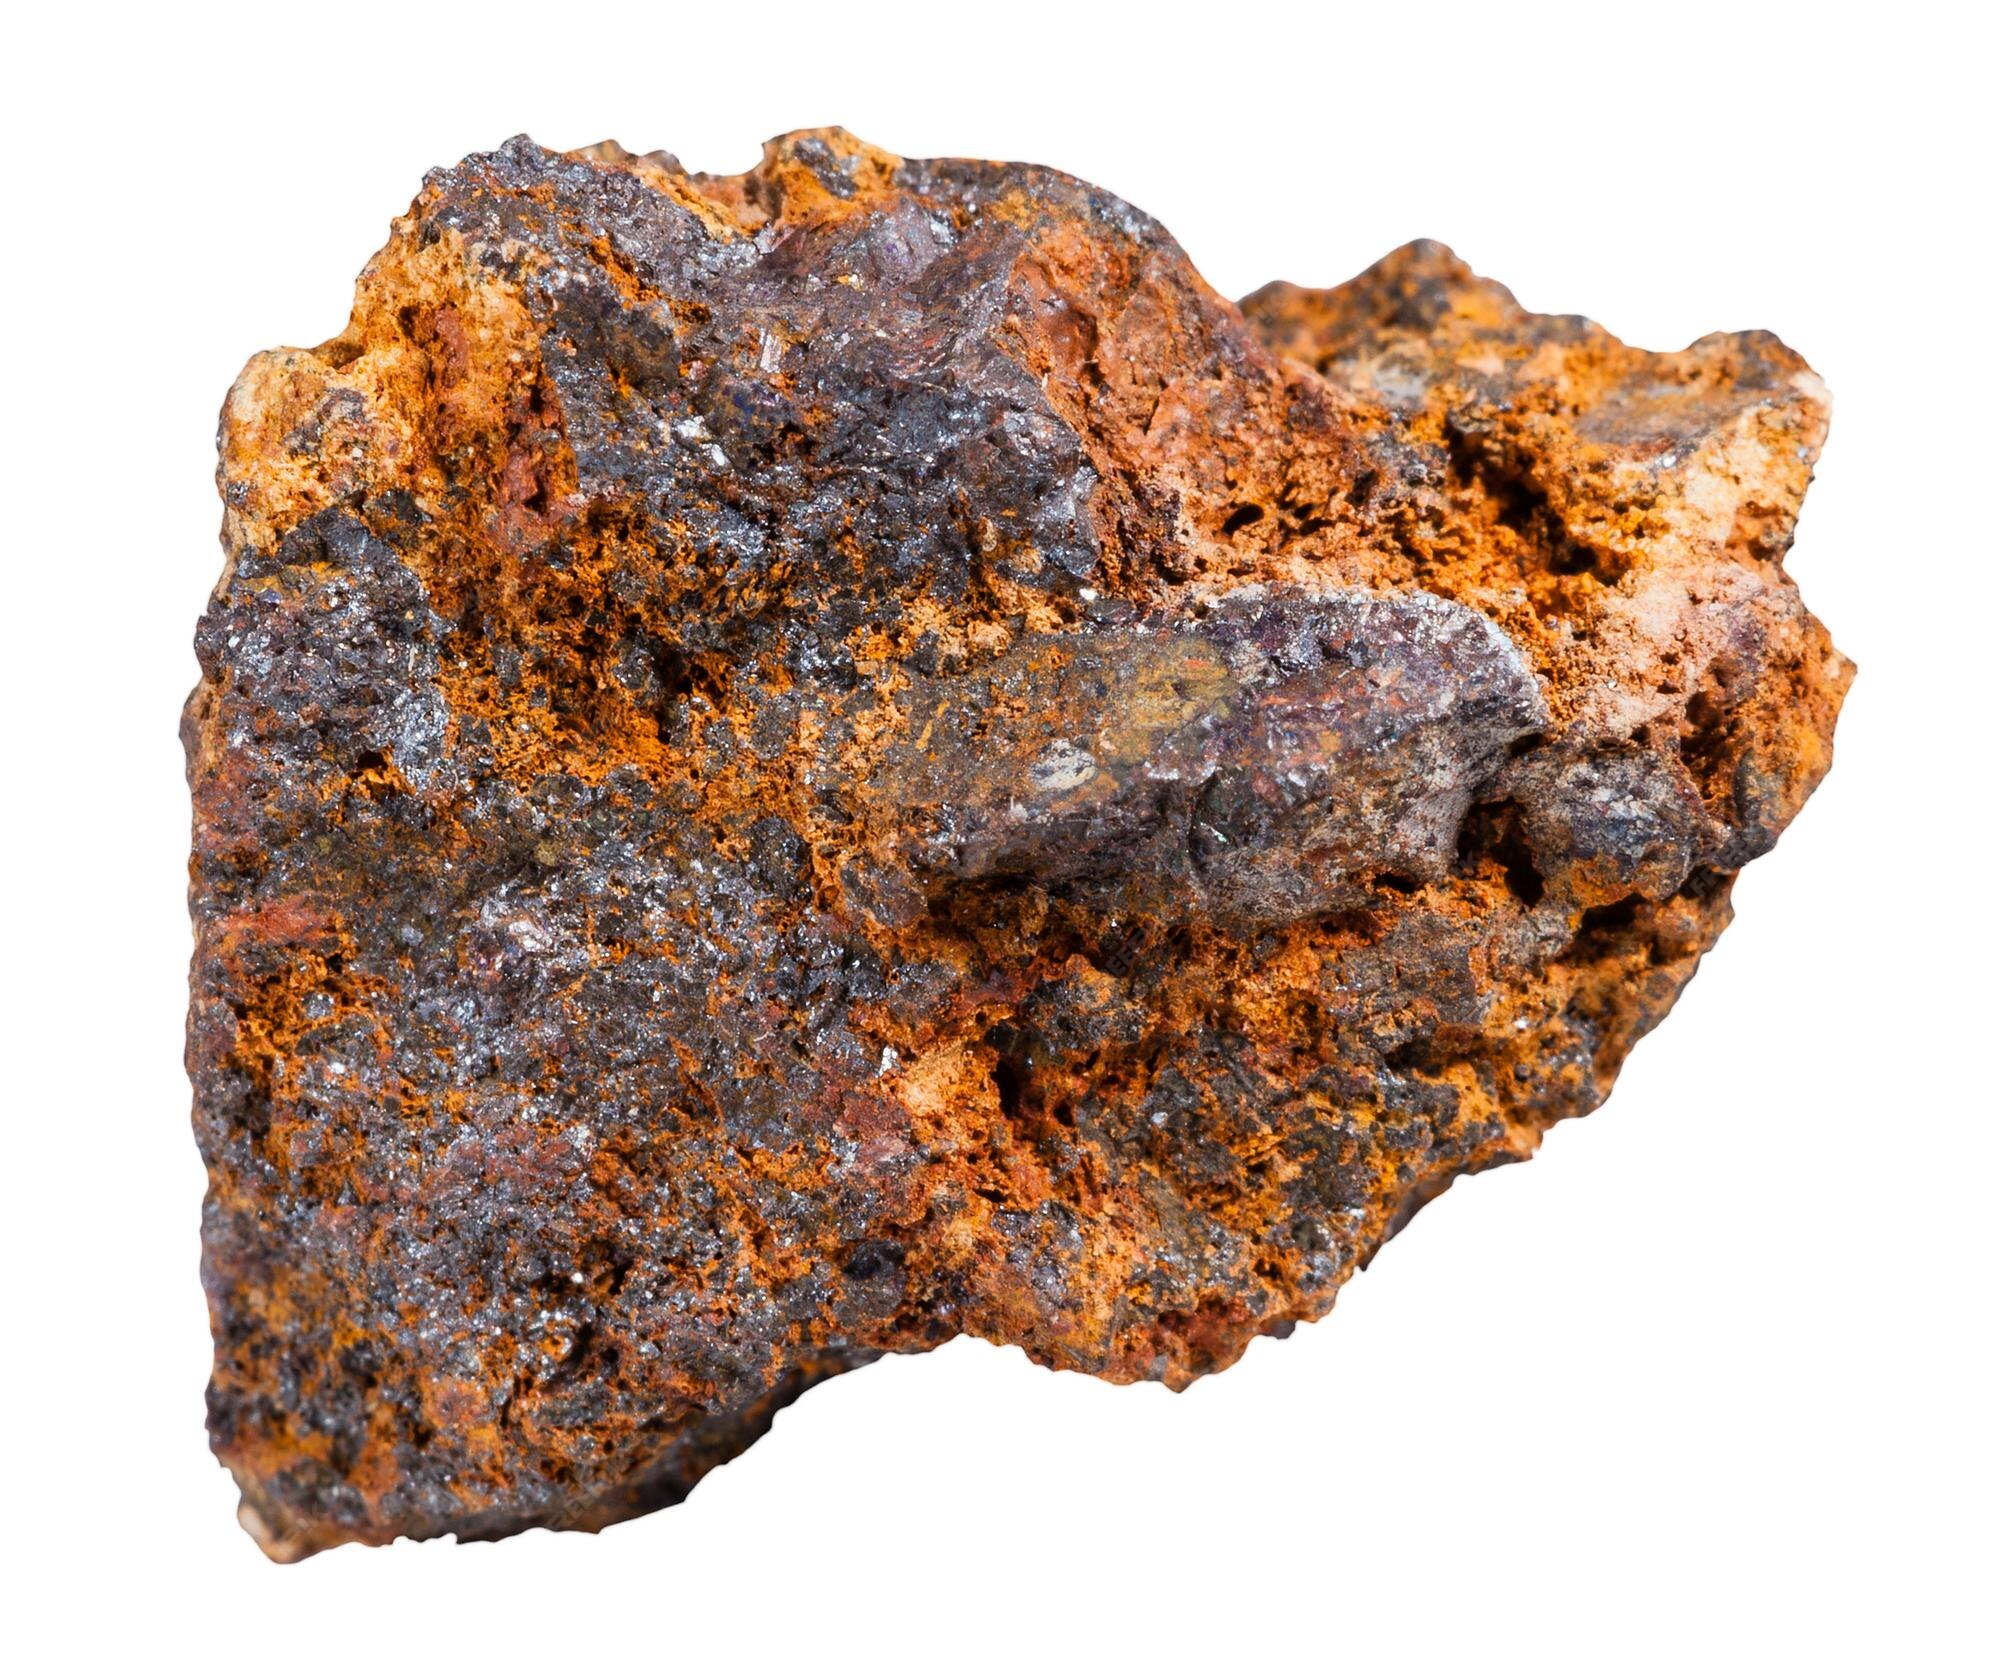
\includegraphics[width=\linewidth,height=3cm,keepaspectratio]{images/hematita.jpg}
      \caption{Hematita (Fe$_2$O$_3$)}
    \end{subfigure}\hfill
    \begin{subfigure}{0.30\linewidth}
      \centering
      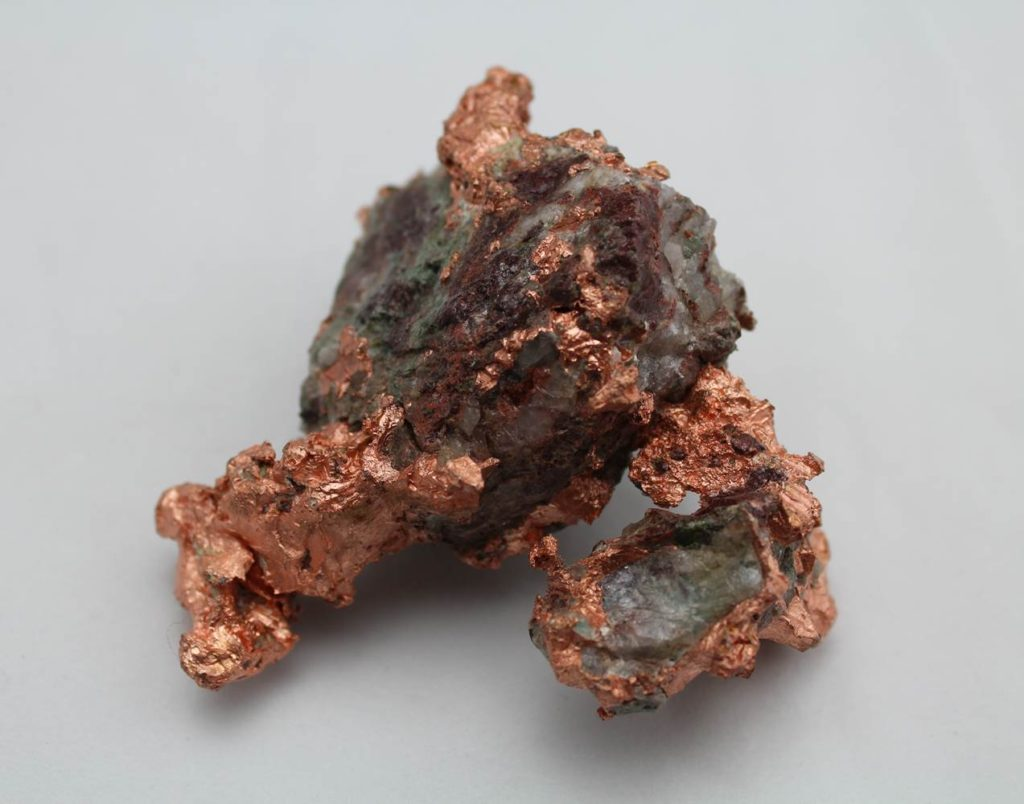
\includegraphics[width=\linewidth,height=3cm,keepaspectratio]{images/cobre.jpg}
      \caption{Cobre (Cu)}
    \end{subfigure}
  \end{figure}
\end{frame}


\begin{frame}{Ejemplos de sólidos cristalinos (carbonatos y otros)}
  \begin{itemize}
    \item \textbf{Calcita (CaCO$_3$)} — trigonal, muy común en rocas sedimentarias.
    \item \textbf{Aragonito (CaCO$_3$)} — polimorfo de la calcita, sistema ortorrómbico.
    \item \textbf{Dolomita (CaMg(CO$_3$)$_2$)} — sistema trigonal.
    \item \textbf{Yeso (CaSO$_4\cdot$2H$_2$O)} — monoclinico, mineral blando.
    \item \textbf{Fluorita (CaF$_2$)} — cúbica, fluorescente bajo luz UV.
  \end{itemize}
\end{frame}

\begin{frame}{Ejemplos de sólidos cristalinos (carbonatos y otros)}
  \begin{figure}
    \centering
    % Primera fila
    \begin{subfigure}{0.30\linewidth}
      \centering
      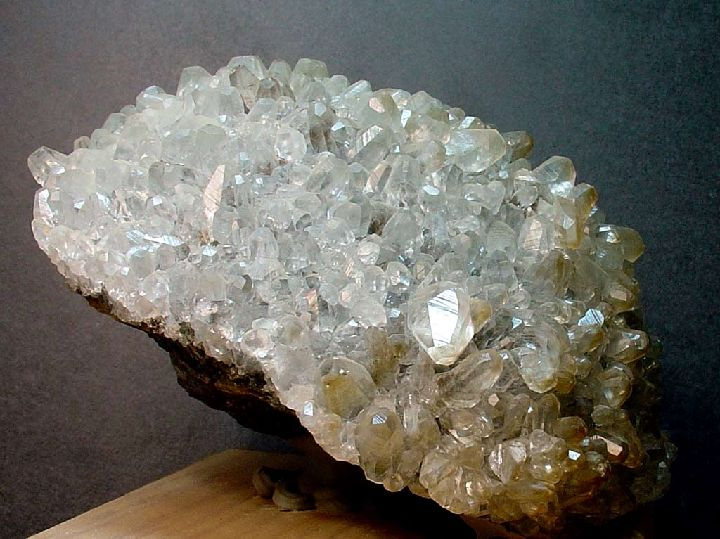
\includegraphics[width=\linewidth,height=3cm,keepaspectratio]{images/calcita.JPG}
      \caption{Calcita (CaCO$_3$)}
    \end{subfigure}\hfill
    \begin{subfigure}{0.30\linewidth}
      \centering
      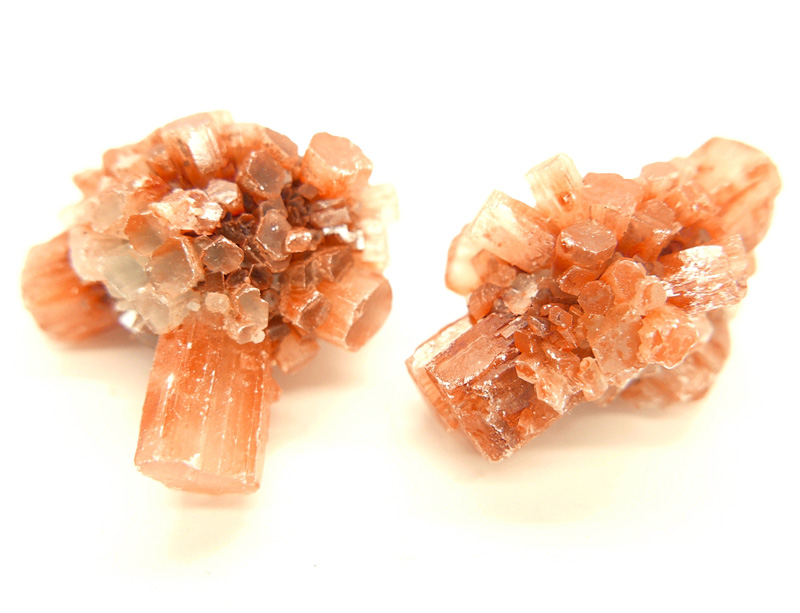
\includegraphics[width=\linewidth,height=3cm,keepaspectratio]{images/aragonito.jpg}
      \caption{Aragonito (CaCO$_3$)}
    \end{subfigure}\hfill
    \begin{subfigure}{0.30\linewidth}
      \centering
      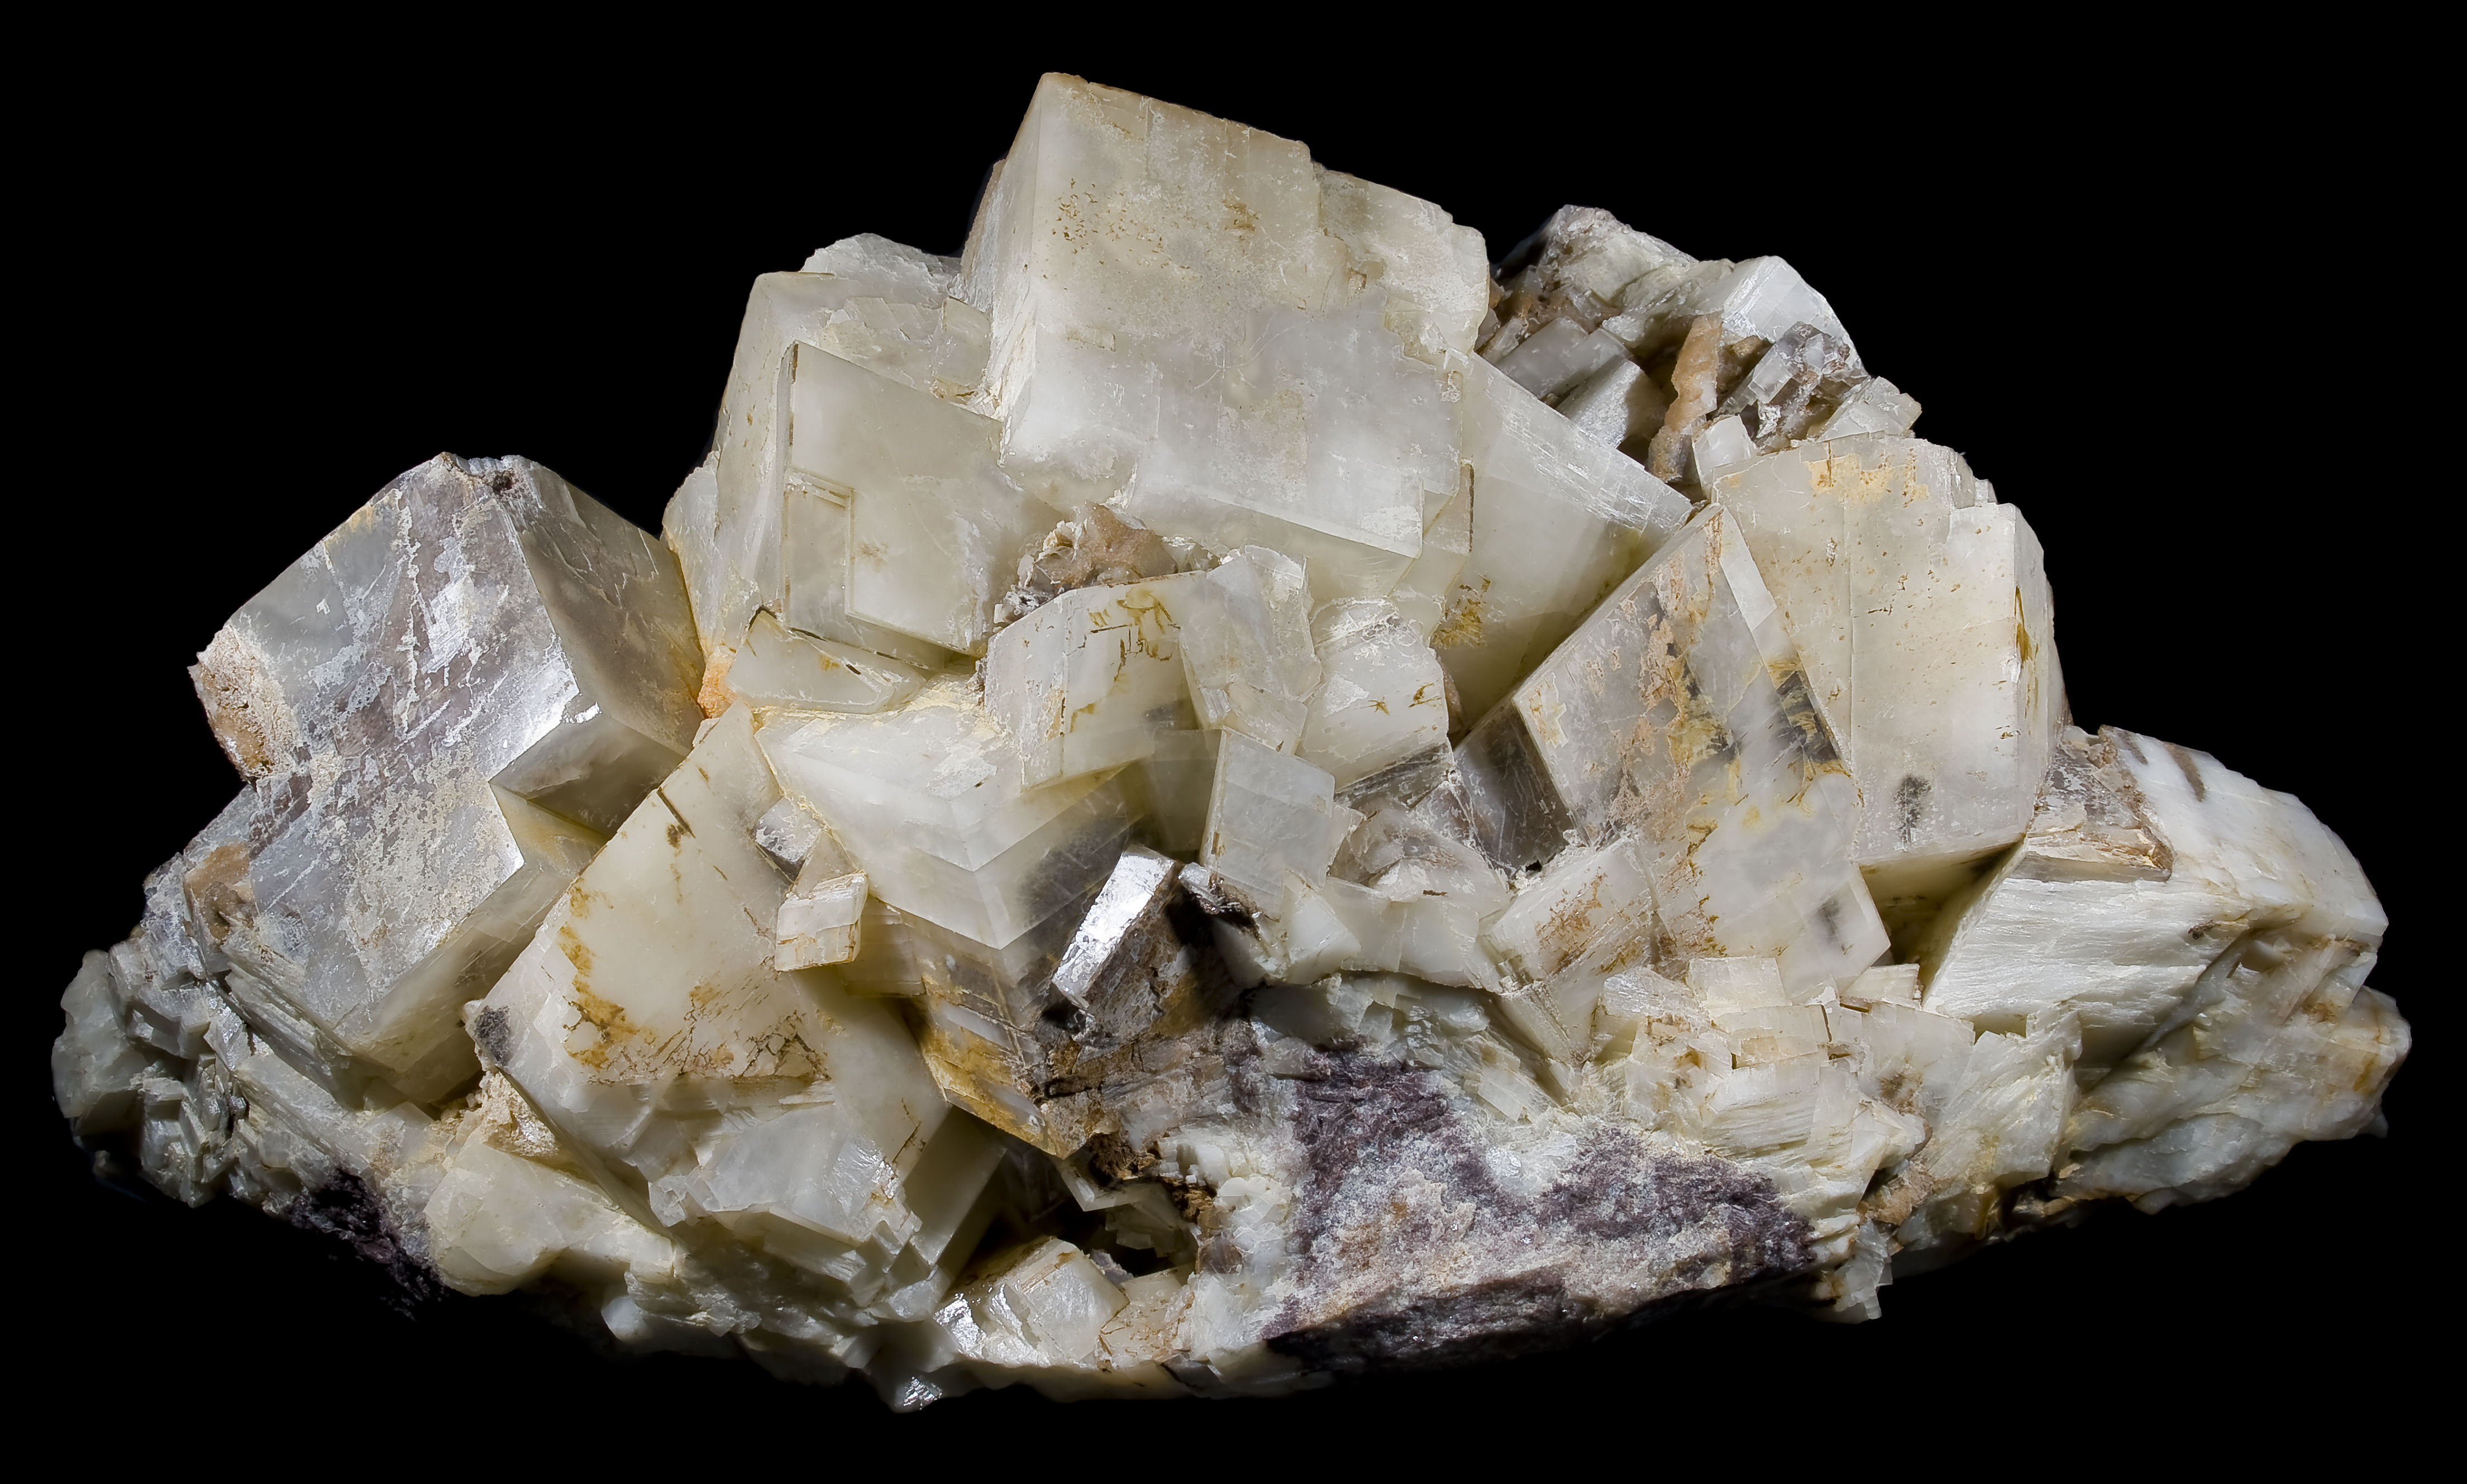
\includegraphics[width=\linewidth,height=3cm,keepaspectratio]{images/dolomita.jpg}
      \caption{Dolomita (CaMg(CO$_3$)$_2$)}
    \end{subfigure}

    \vspace{0.3cm}

    % Segunda fila
    \begin{subfigure}{0.30\linewidth}
      \centering
      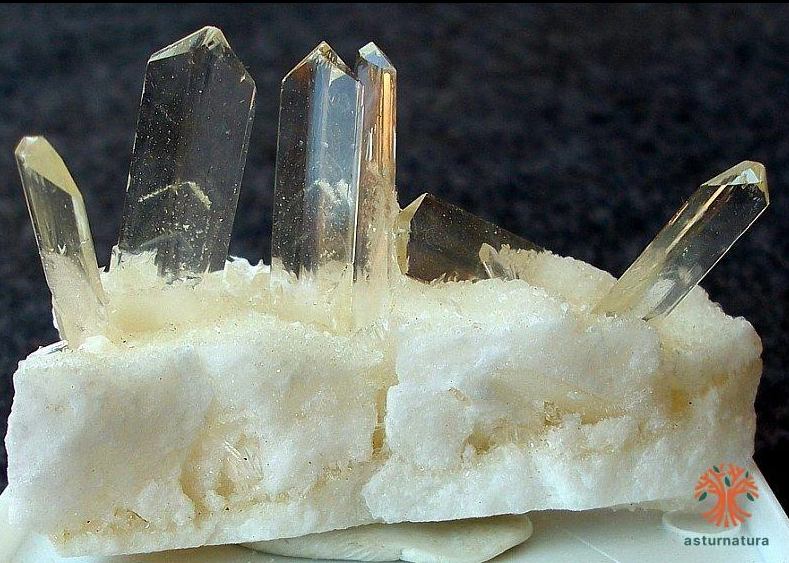
\includegraphics[width=\linewidth,height=3cm,keepaspectratio]{images/yeso.png}
      \caption{Yeso (CaSO$_4\cdot$2H$_2$O)}
    \end{subfigure}\hfill
    \begin{subfigure}{0.30\linewidth}
      \centering
      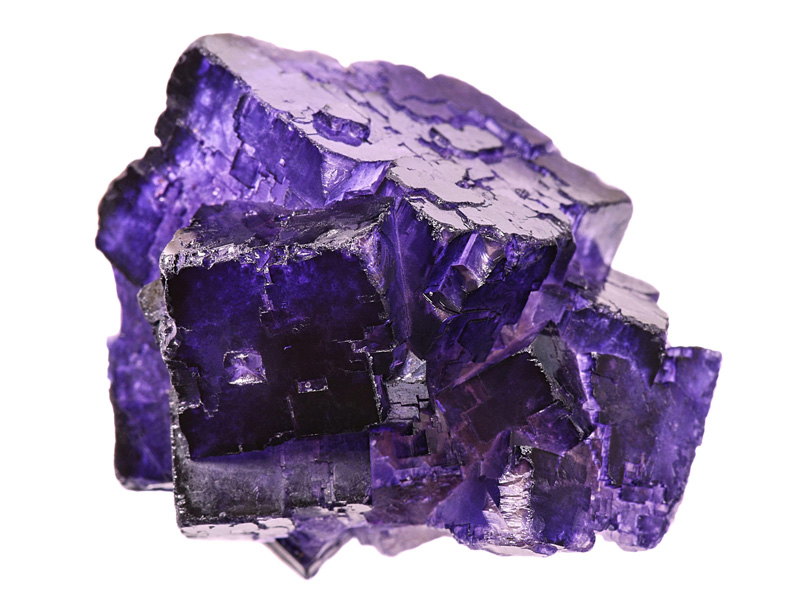
\includegraphics[width=\linewidth,height=3cm,keepaspectratio]{images/fluorita.jpg}
      \caption{Fluorita (CaF$_2$)}
    \end{subfigure}
  \end{figure}
\end{frame}


\begin{frame}{Ejemplos de sólidos cristalinos (tecnológicos)}
  \begin{itemize}
    \item \textbf{Silicio (Si)} — base de la microelectrónica, estructura cúbica tipo diamante.
    \item \textbf{Germanio (Ge)} — semiconductor con red cúbica tipo diamante.
    \item \textbf{ZnS (Blenda)} — cúbica, usada en optoelectrónica.
    \item \textbf{GaAs} — cristal semiconductores, red cúbica tipo zincblenda.
    \item \textbf{LiFePO$_4$} (fosfato de hierro-litio)— catodo en baterías de litio.
  \end{itemize}
\end{frame}

\begin{frame}{Ejemplos de sólidos cristalinos (tecnológicos)}
  \begin{figure}
    \centering
    % Primera fila
    \begin{subfigure}{0.30\linewidth}
      \centering
      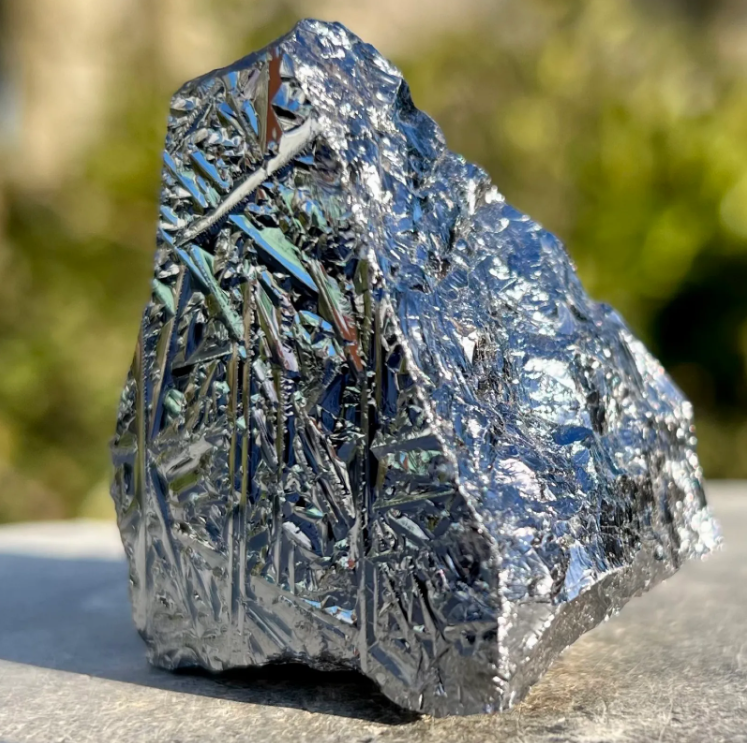
\includegraphics[width=\linewidth,height=3cm,keepaspectratio]{images/silicio.png}
      \caption{Silicio (Si)}
    \end{subfigure}\hfill
    \begin{subfigure}{0.30\linewidth}
      \centering
      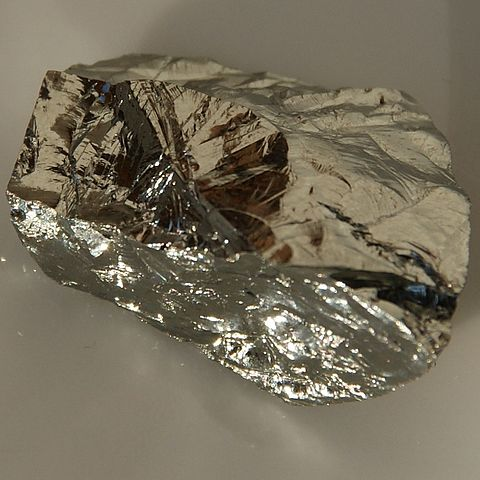
\includegraphics[width=\linewidth,height=3cm,keepaspectratio]{images/germanio.jpg}
      \caption{Germanio (Ge)}
    \end{subfigure}\hfill
    \begin{subfigure}{0.30\linewidth}
      \centering
      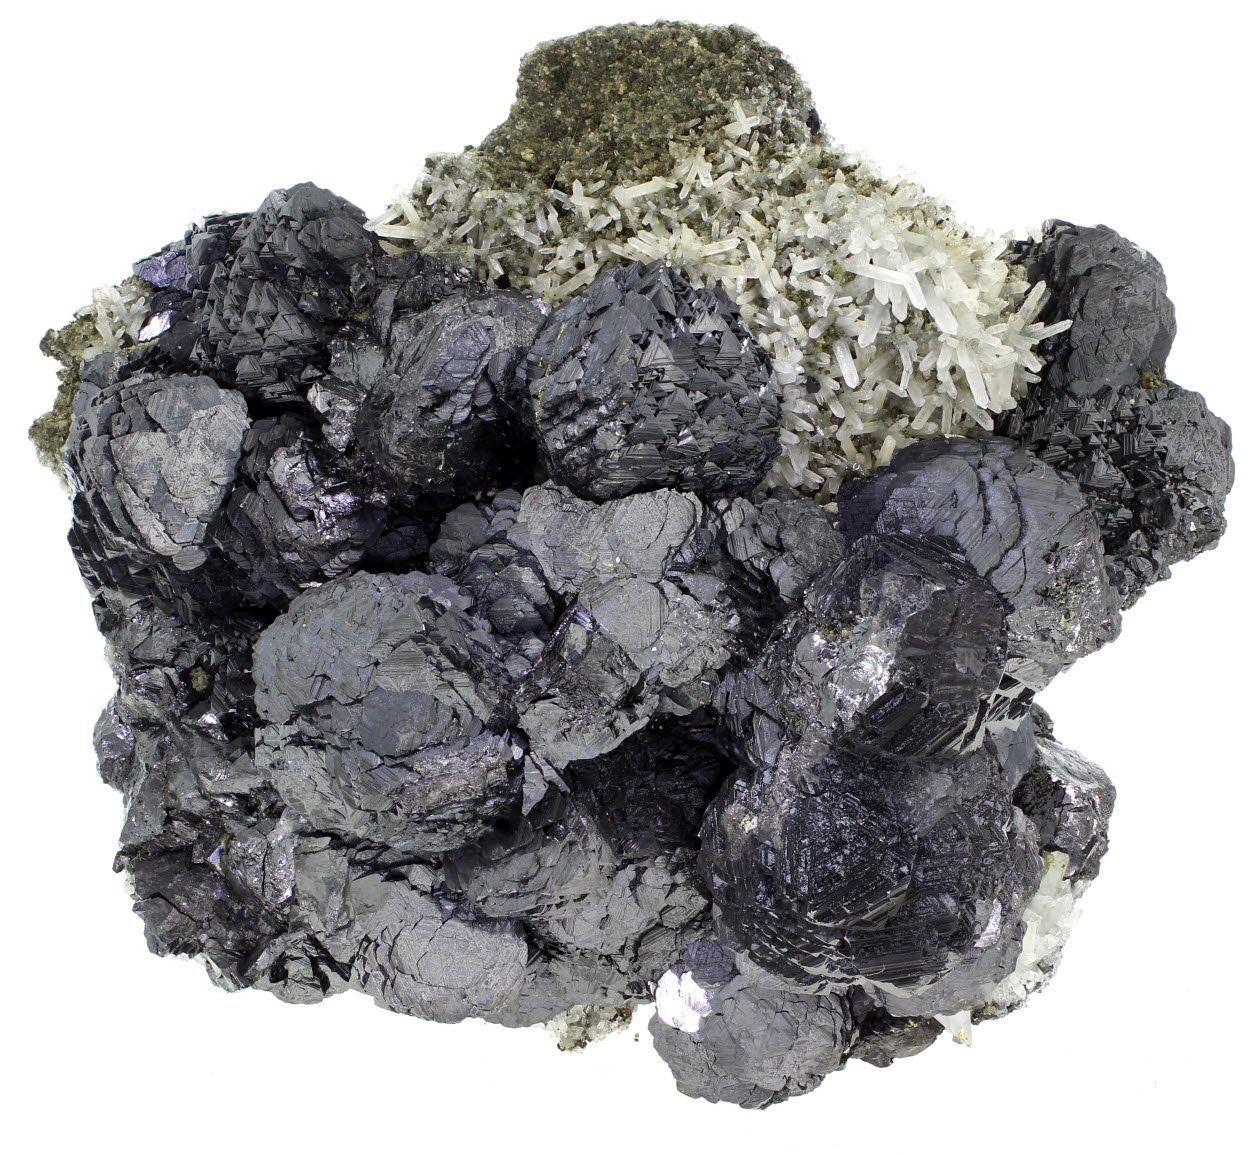
\includegraphics[width=\linewidth,height=3cm,keepaspectratio]{images/zns.jpg}
      \caption{Blenda (ZnS)}
    \end{subfigure}

    \vspace{0.3cm}

    % Segunda fila
    \begin{subfigure}{0.30\linewidth}
      \centering
      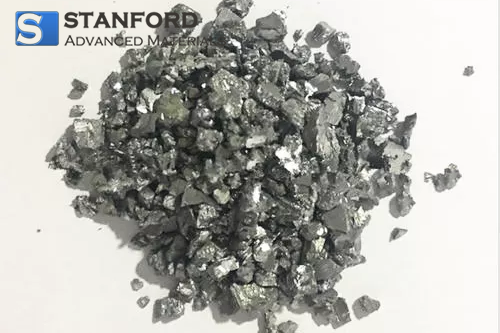
\includegraphics[width=\linewidth,height=3cm,keepaspectratio]{images/gaas.png}
      \caption{Arseniuro de galio (GaAs)}
    \end{subfigure}
  \end{figure}
\end{frame}


\begin{frame}{Red cristalina}
  \begin{itemize}
    \item Forma sólida de como se ordenan y empaquetan los átomos, moléculas o iones. Se empaquetan de forma ordenada con patrones de repeticiones en el espacio. 
    \item La \underline{celda unitaria} reproduce la red completa trasladada en las 3 dimesiones repetidamente. Siempre es la misma para cualquier estructura cristalina dada.
    \item Está definida por parámetros $a$, $b$ y $c$ y por sus ángulos entre los ejes $\alpha$, $\beta$, $\gamma$
  \end{itemize}
\end{frame}
    
\begin{frame}{Red cristalina}
  \begin{figure}
    \centering
    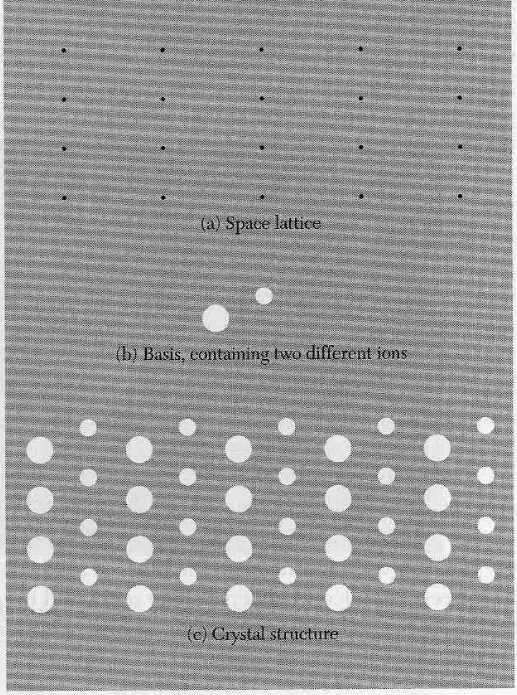
\includegraphics[width=0.35\linewidth]{images/estructura_cristalina}
    \caption{La estructura cristalina se forma al añadir la base (b) a cada punto de la red espacial (a), obteniendo así la red cristalina (c).}
  \end{figure}
\end{frame}

% --- Celda unitaria (concepto + vectores de red)
\begin{frame}{Celda unitaria y vectores de red}
  \begin{columns}
    \column{0.58\textwidth}
    \begin{itemize}
      \item La \textbf{celda unitaria} es el bloque más pequeño que, por traslaciones, reconstruye todo el cristal.
      \item Está definida por sus parámetros: \(a,b,c\) y \(\alpha,\beta,\gamma\).
      \item Matemáticamente, se describe mediante tres \textbf{vectores primitivos de red}:
        \[
          \vec{R} = n_1\vec{a}_1 + n_2\vec{a}_2 + n_3\vec{a}_3, 
          \quad n_i \in \mathbb{Z}
        \]
      \item La \textbf{base} (átomos) se coloca en posiciones fraccionarias dentro de la celda.
    \end{itemize}
    
    \column{0.42\textwidth}
      \centering
      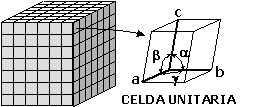
\includegraphics[width=\linewidth]{images/celda_unitaria.png}
      \captionof{figure}{Parámetros de red y vectores primitivos de una celda genérica.}
  \end{columns}
\end{frame}

%%%%%%%%%%%%%%%%%%%%%%%%%%%%%%%%%%%%%

\begin{frame}{}
 \begin{figure}
    \centering
    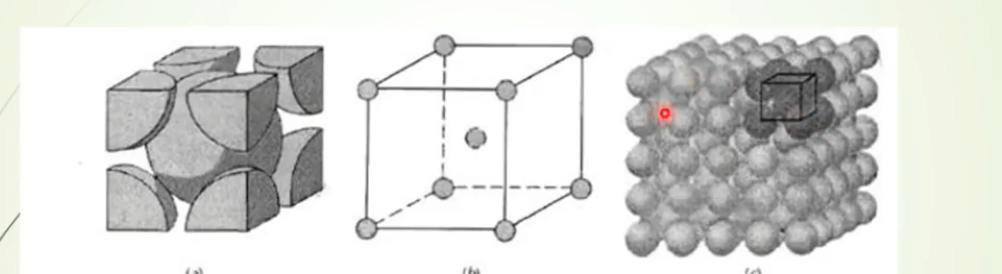
\includegraphics[width=0.8\linewidth]{images/celda_unitaria_2}
    \caption{Mismas propiedades y características que todo el sólido completo.}
 \end{figure}
\end{frame}

%%%%%%%%%%%%%%%%%%%%%%%%%%%%%%%%%%%%%





% --- Factor de empaquetamiento atómico (FEA)
\begin{frame}{Factor de empaquetamiento atómico (APF)}
  \begin{itemize}
    \item El \textbf{FEA} mide la fracción del volumen de la celda unitaria que está ocupada por los átomos.
      \[
        APF = \frac{\text{Volumen de los átomos en la celda}}{\text{Volumen de la celda unitaria}}
      \]
      
      \[ APF = \frac{ N_{atomos} V_{atomos} }{V_{celda unitaria}} \] 
    \item Valores típicos:
      \begin{itemize}
        \item Cúbica simple (SC): \(APF \approx 0.52\).
        \item Cúbica centrada en el cuerpo (BCC): \(APF \approx 0.68\).
        \item Cúbica centrada en las caras (FCC): \(APF \approx 0.74\) 
      \end{itemize}
    \item El FEA influye en la \textbf{densidad} y \textbf{propiedades mecánicas} de los sólidos.
  \end{itemize}
\end{frame}

% --- Sistemas cristalinos (con dos columnas)
\begin{frame}{Sistemas cristalinos}
  \begin{columns}
    % Columna izquierda: texto
    \column{0.55\textwidth}
      \begin{itemize}
        \item Existen \textbf{7 sistemas cristalinos}, definidos por relaciones entre $a,b,c$ y los ángulos $\alpha,\beta,\gamma$:
        \begin{enumerate}
          \item Triclínico
          \item Monoclínico
          \item Ortorrómbico
          \item Tetragonal
          \item Trigonal (romboédrico)
          \item Hexagonal
          \item Cúbico
        \end{enumerate}
        \item Cada sistema admite distintos tipos de \textbf{centrado de celda}.
      \end{itemize}

    % Columna derecha: imagen
    \column{0.45\textwidth}
      \centering
      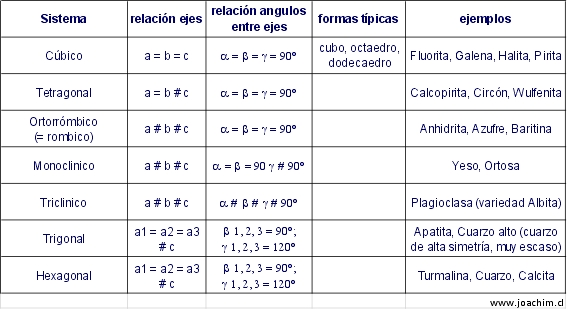
\includegraphics[width=\linewidth]{images/sistemas_cristalinos.jpeg}
      \captionof{figure}{Representación de las 7 redes  cristalinas.}
  \end{columns}
\end{frame}


% --- Redes de Bravais (vistoso con 2 columnas)
\begin{frame}{Redes de Bravais}
  \begin{columns}
    % Columna izquierda
    \column{0.55\textwidth}
      \begin{itemize}
        \item Combinando los \textbf{7 sistemas cristalinos} con los posibles \textbf{centrados}:
          \[
            7 \;\;\;\longrightarrow\;\;\; 14 \; \text{redes de Bravais}
          \]
        \item Tipos de centrado:
          \begin{itemize}
            \item \textbf{P}: Primitiva.
            \item \textbf{I}: Centrada en el cuerpo.
            \item \textbf{F}: Centrada en las caras.
            \item \textbf{C}: Centrada en una bases.
          \end{itemize}
        \item Ejemplos:
          \begin{itemize}
            \item Sistema cúbico $\to$ P, I, F (3 redes).
            \item Sistema ortorrómbico $\to$ P, C, I, F (4 redes).
          \end{itemize}
      \end{itemize}

    % Columna derecha
    \column{0.45\textwidth}
      \centering
      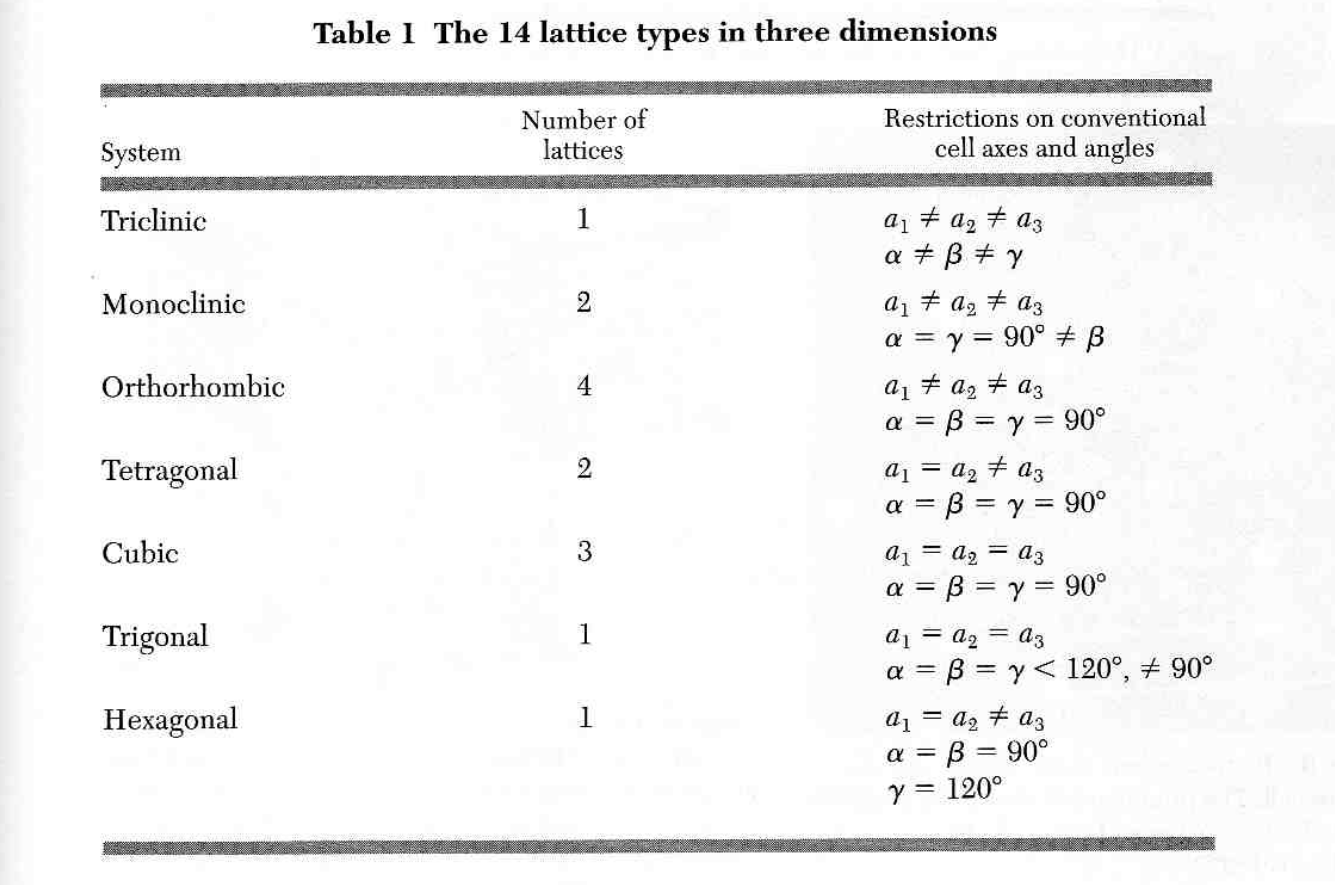
\includegraphics[width=\linewidth]{images/bravais_14.png}
      \captionof{figure}{Las 14 redes de Bravais en 3D.}
  \end{columns}
\end{frame}


 \section{Red ortorrómbica centrada en las bases}
    
    \frame{\sectionpage}

% --- Introducción a la red ortorrómbica C
\begin{frame}{Ortorrómbica centrada en las bases (C)}
  \begin{itemize}
    \item Forma parte del \textbf{sistema ortorrómbico}: $a \neq b \neq c$ y $\alpha = \beta = \gamma = 90^\circ$.
    \item En la variante \textbf{C-centrada} (centrada en las bases), además de los vértices hay puntos de red en el centro de dos caras opuestas (paralelas al eje $c$).
    \item Es una de las \textbf{14 redes de Bravais}.
    \item Se utiliza para describir materiales cuyas propiedades derivan de esta simetría particular.
  \end{itemize}
  \vspace{0.3cm}
  \centering
  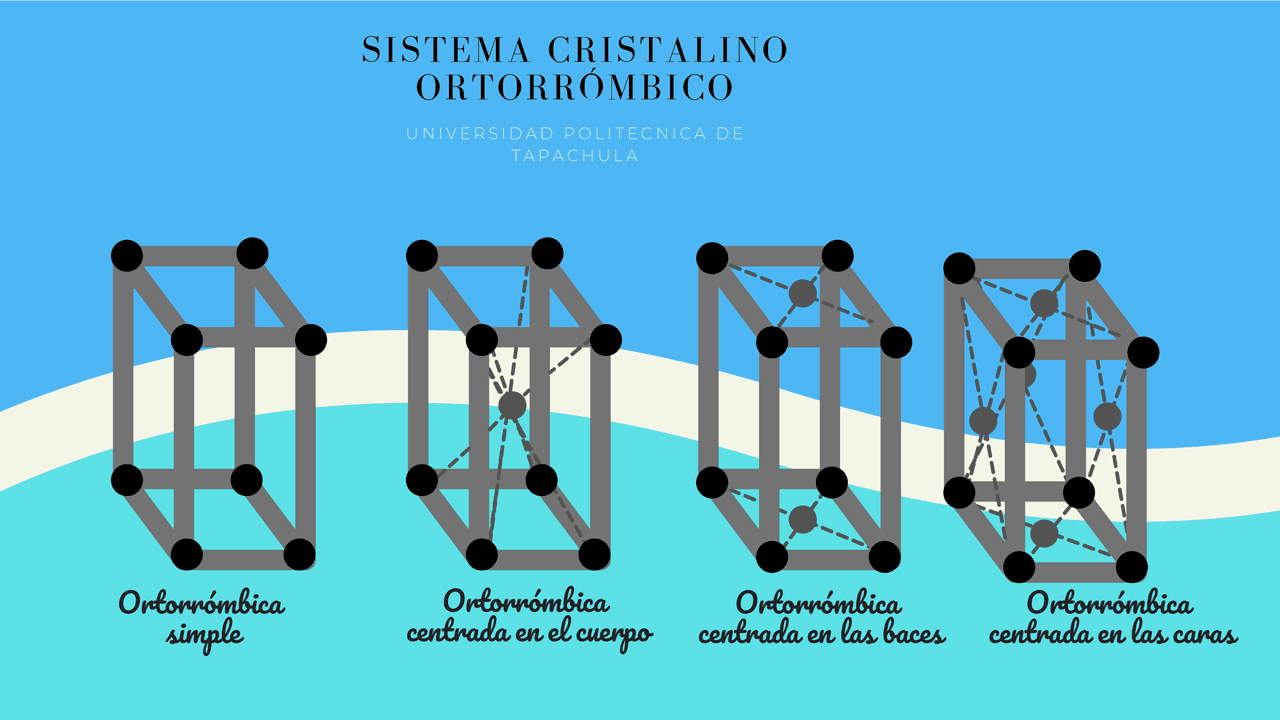
\includegraphics[width=0.4\linewidth]{images/ortorrombica_C.png}
  \captionof{figure}{Esquema de celda ortorrómbica C-centrada.}
\end{frame}

    
\subsection{Ejemplos}

    \frame{\subsectionpage}

%==================== EJEMPLO 1: α-URANIO ====================

%==================== EJEMPLO 1: α-URANIO ====================

\begin{frame}{Ejemplo 1 — $\alpha$-Uranio: datos cristalográficos}
  \begin{itemize}
    \item \textbf{Composición química:} U (elemento).
    \item \textbf{Sistema cristalino:} Ortorrómbico, $\alpha=\beta=\gamma=90^\circ$.
    \item \textbf{Tipo de celda:} C-centrada (oC).
    \item \textbf{Grupo espacial:} Cmcm (No.\,63).
    \item \textbf{Parámetros típicos a 298 K:}
      \[
        a \approx 2.84,\quad
        b \approx 5.87,\quad
        c \approx 4.96
      \]
    \item \textbf{Motivo estructural:} capas corrugadas de U con enlaces direccionales.
  \end{itemize}
  \vspace{0.3cm}
  \centering
  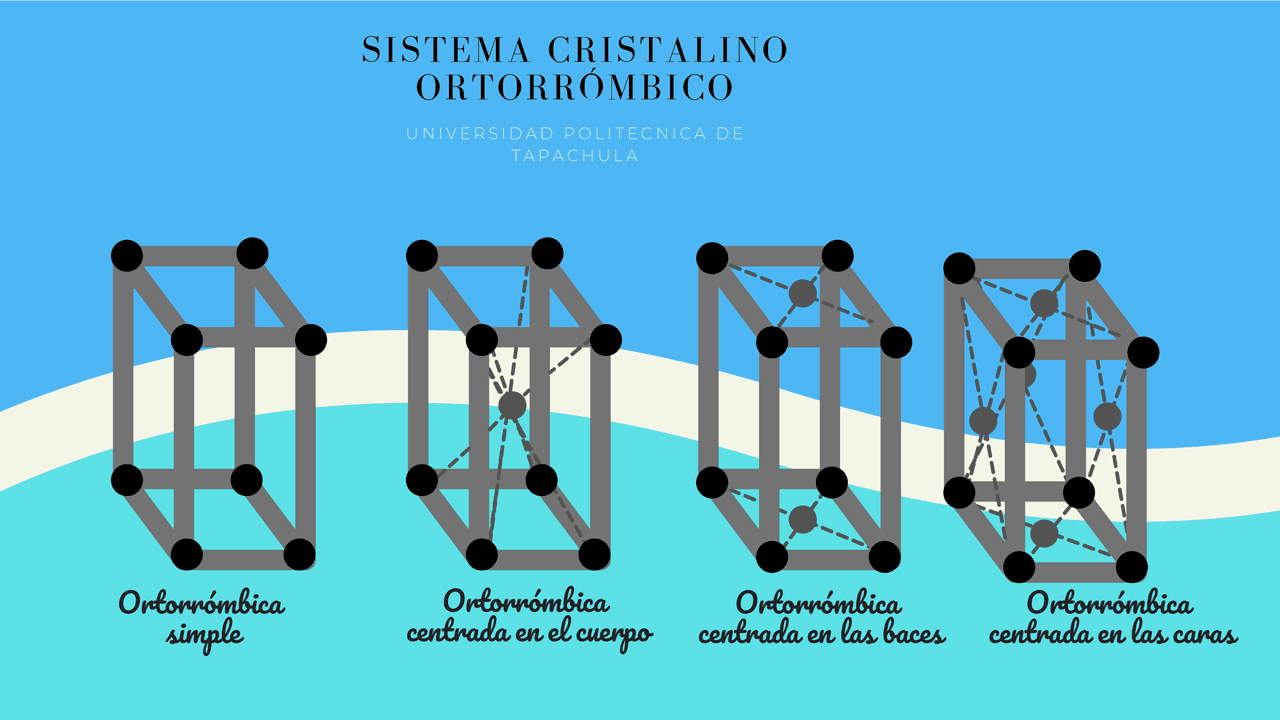
\includegraphics[width=0.45\linewidth]{images/ortorrombica_C.png}
  \captionof{figure}{Estructura ortorrómbica C-centrada del $\alpha$-U (Cmcm).}
\end{frame}

\begin{frame}{Ejemplo 1 — $\alpha$-Uranio: propiedades \& aplicaciones}
  \begin{itemize}
    \item \textbf{Propiedades:} metal denso, anisotropía marcada (térmica y mecánica), varias transiciones de fase.
    \item \textbf{Estructura:} la simetría Cmcm (oC) favorece anisotropía en dilatación y elasticidad.
    \item \textbf{Aplicaciones:} materiales nucleares (combustible, aleaciones); interés bajo presión/temperatura.
  \end{itemize}
  \vspace{0.3cm}
  \centering
  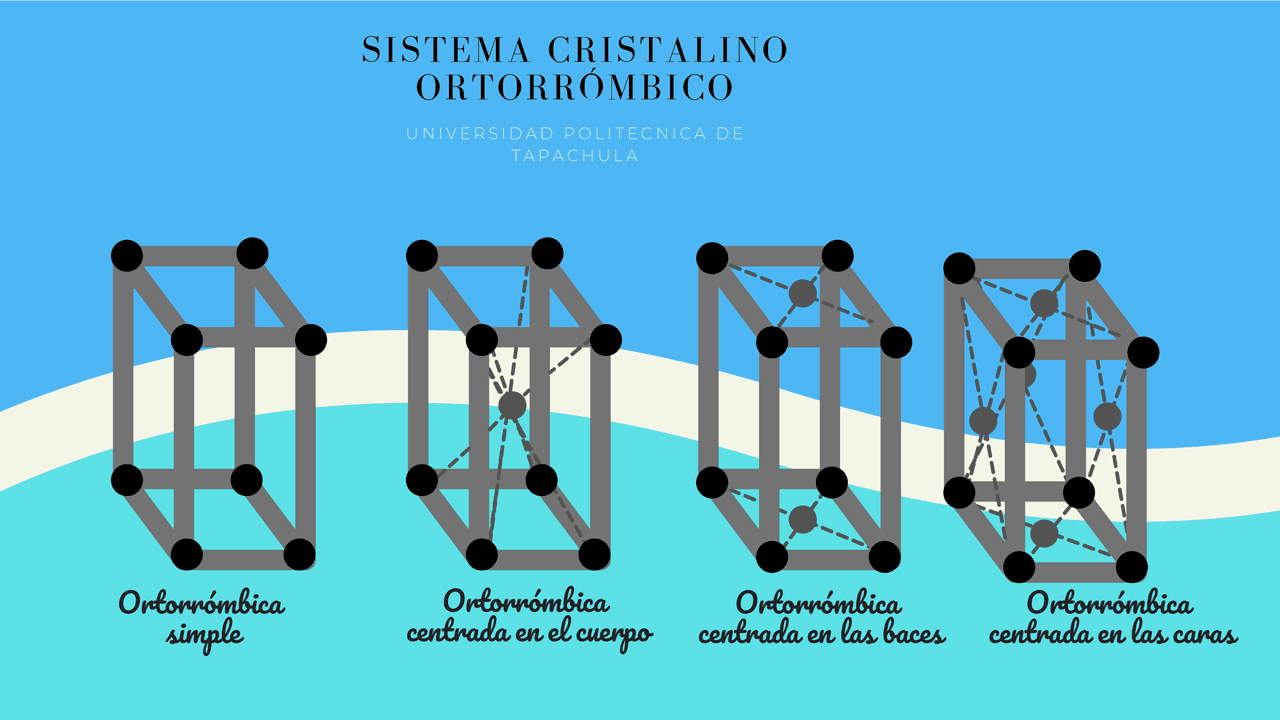
\includegraphics[width=0.55\linewidth]{images/ortorrombica_C.png}
  \captionof{figure}{Vista esquemática por capas del $\alpha$-U resaltando anisotropía.}
\end{frame}

%==================== EJEMPLO 2: α-GALIO ====================

\begin{frame}{Ejemplo 2 — $\alpha$-Galio: datos cristalográficos}
  \begin{itemize}
    \item \textbf{Composición química:} Ga (elemento).
    \item \textbf{Sistema cristalino:} Ortorrómbico, $\alpha=\beta=\gamma=90^\circ$.
    \item \textbf{Tipo de celda:} C-centrada (oC).
    \item \textbf{Grupo espacial:} Cmca (No.\,64).
    \item \textbf{Parámetros típicos (RT):}
      \[
        a \approx 4.52,\quad
        b \approx 7.66,\quad
        c \approx 4.53
      \]
    \item \textbf{Motivo estructural:} “molecular-metálico” (enlaces Ga–Ga cortos + red extendida).
  \end{itemize}
  \vspace{0.3cm}
  \centering
  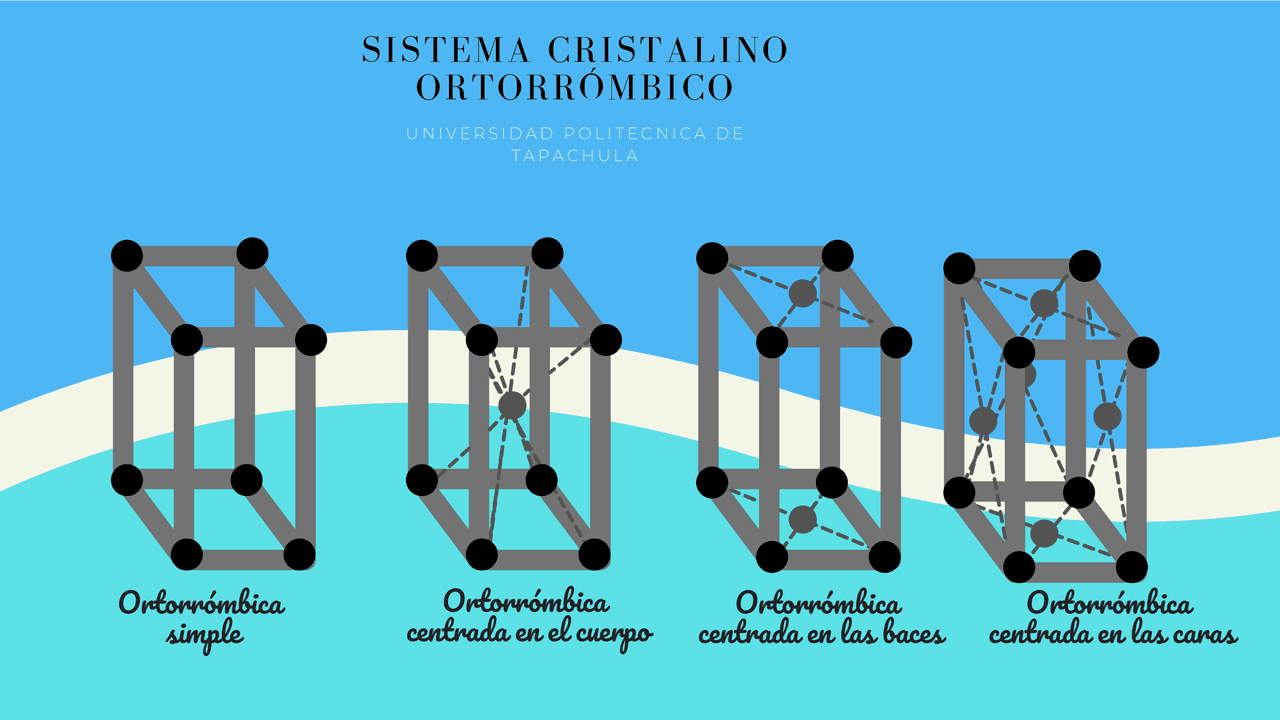
\includegraphics[width=0.45\linewidth]{images/ortorrombica_C.png}
  \captionof{figure}{Estructura ortorrómbica C-centrada del $\alpha$-Ga (Cmca).}
\end{frame}

\begin{frame}{Ejemplo 2 — $\alpha$-Galio: propiedades \& aplicaciones}
  \begin{itemize}
    \item \textbf{Propiedades:} punto de fusión muy bajo (29.8 {$\circ$}C), mojabilidad elevada, expansión al solidificar.
    \item \textbf{Estructura:} la Cmca (oC) con pares Ga–Ga cortos explica su comportamiento “meta-molecular”.
    \item \textbf{Aplicaciones:} soldaduras de baja T, metales líquidos en microfluídica, base de semiconductores (GaAs, GaN).
  \end{itemize}
  \vspace{0.3cm}
  \centering
  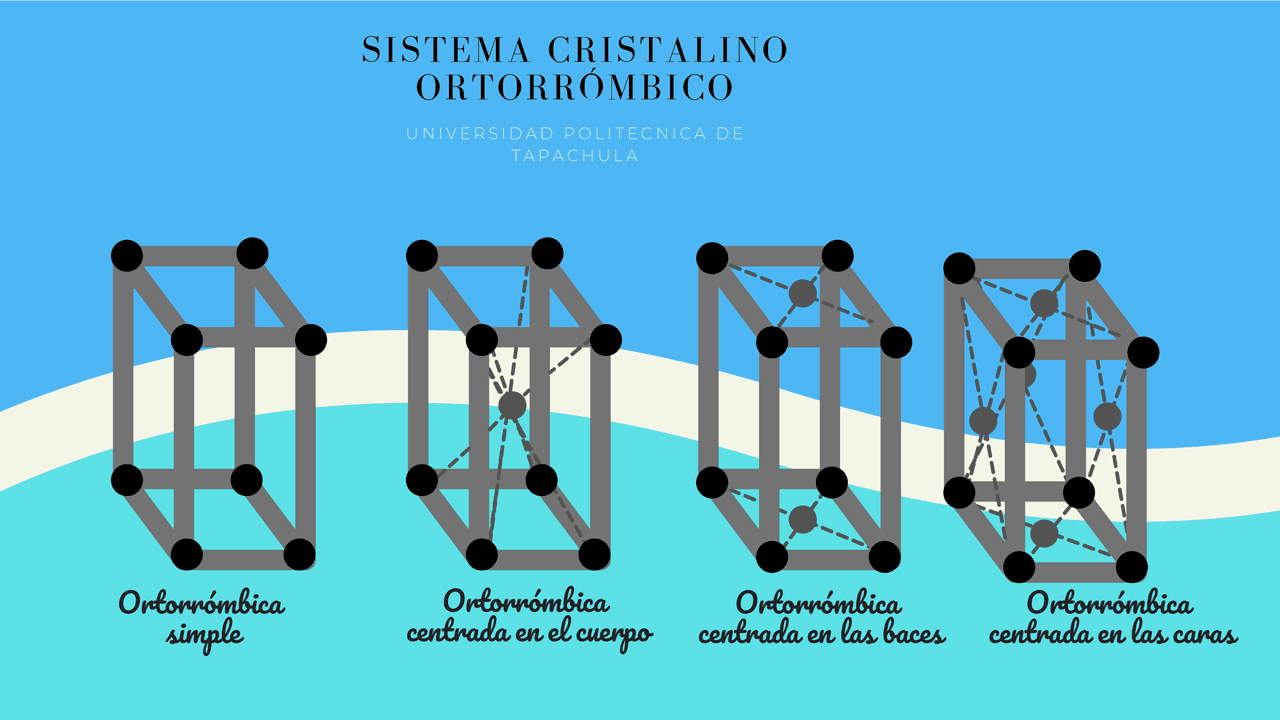
\includegraphics[width=0.55\linewidth]{images/ortorrombica_C.png}
  \captionof{figure}{Esquema de enlaces Ga–Ga cortos y red extendida en $\alpha$-Ga.}
\end{frame}




    
    \section*{Referencias} %You can remove this if you do not want to use it
        \nocite{Djairo} \nocite{PhilPanof} \nocite{Fleming} \nocite{Shankar}
        \begin{frame}{References}
            \printbibliography
        \end{frame}

    \section{}
    \begin{frame}{}
        \centering
            \Huge\bfseries
        \textcolor{orange}{The End}
    \end{frame}
\end{document}
